\documentclass[10pt,a4paper]{article}
\usepackage[utf8]{inputenc}
\usepackage[german]{babel}
\usepackage[T1]{fontenc}
\usepackage{amsmath}
\usepackage{amsfonts}
\usepackage{amssymb}
\usepackage{graphicx}
\usepackage{lmodern}
\usepackage{bm}
\usepackage{tikz}
\usepackage[margin=1.2in]{geometry}

\DeclareMathOperator{\atan}{atan}

\author{Lars Schiller}
\begin{document}

\title{Doc of PathPlanning Approaches for GeckoBot}

\maketitle
\tableofcontents

\section{Predicting the next pose of the robot}
\subsection{Modeling of Soft Bending Actuator}

\begin{itemize}
	\item Einführung virtueller Längen, um größeren Bereich erreichen zu können, und dennoch die Annahme von \textsl{Constant curvature} nutzen zu können.
	\item Weil Sehr effektiv zu rechnen.
\end{itemize}

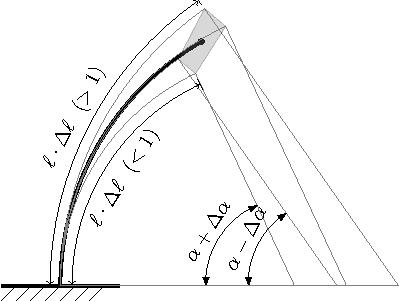
\includegraphics[scale=1]{pics/Virtual_length/virtual_length.pdf}



\subsection{Modeling of the robot}

	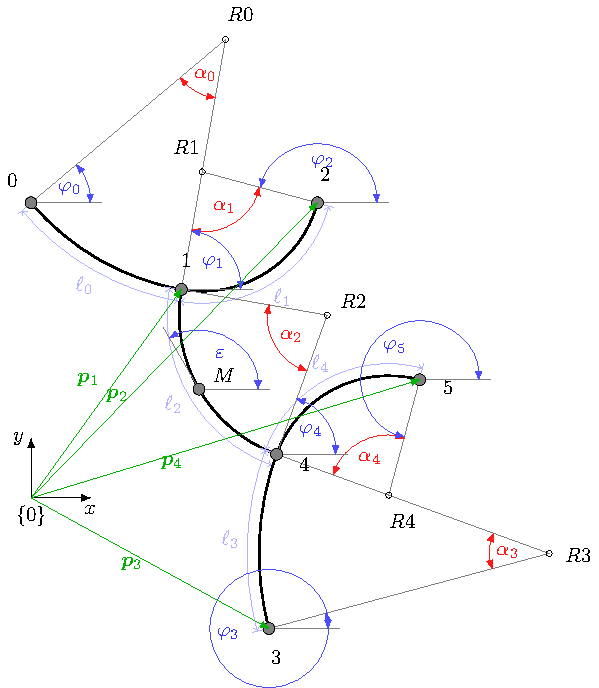
\includegraphics[scale=1]{pics/general_model/model_plain.pdf}

	\begin{itemize}
		\item Zustands- und Eingangsgrößen:
		$$
		\bm{x} = \left[~\bm{\alpha}~\bm{\ell}~\varepsilon~\right],~~~
		\bm{r} = \left[~\bm{\alpha}_{\textnormal{ref}}~\bm{f}~\right]
		$$
		
		\item Innere Spannung:
		$$
		\begin{array}{rcl}
		\sigma(\bm{x}_{k}) 
		&=&  w_\ell\big| \bm{\ell}_{k} - \bm{\ell}_n \big|_2 \\
		&&	+ w_\alpha\big| \bm{\alpha}_{k} - \bm{\alpha}_{\textnormal{ref},k} \big|_2 \\
		&&	+ w_\varphi \big| \textnormal{diag}(\bm{f}_k) ( \bm{\varphi}_{k} - \bm{\varphi}_{k-1}) \big|_2 \\
		\end{array}
		$$
		
		\item Minimale Spannung:
		$$
		\begin{array}{l}
		\displaystyle\min_{\bm{x}_k \in \mathcal{X}} ~ \sigma(\bm{x}_k) \\
		s.~t.~~~
		\big|\big|\textnormal{diag}(\bm{f}_k)(\bm{P}_{k} - \bm{P}_{k-1})\big|\big|_2 = 0
		\end{array}
		$$
		
		\item Folgepose:
		$$
		\bm{\rho}_k = [\bm{x}_k~\bm{P}_k~\bm{f}_k] = \textnormal{fun}_{\mathcal{P}}\left( \bm{r}_k, \bm{\rho}_{k-1} \right)
		$$
		
		\item Das Modell liefert dann eine quasi statische Vorhersage der neuen Ruhelage zu gegebenen Eingangsgrößen:
		
		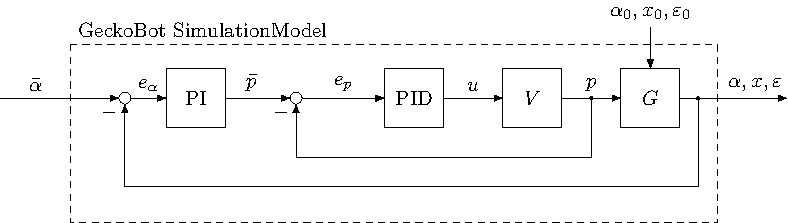
\includegraphics[scale=1]{pics/CtrLoops/GeckoBotModel.pdf}
	\end{itemize}
	


\section{Path Planning with Search Tree}


\subsection{Different Gait Patterns for a curve}

\begin{itemize}
	\item Vom Kinematic Paper sind schon verschieden Laufmuster für Kurven bekannt, basierend auf dem Minimierungsproblem:
	
	\begin{equation}
		\displaystyle\min_{\bm{\alpha} \in \mathcal{A}} ~ \varepsilon(\bm{\alpha})
	\end{equation}
	
	wobei $\bm{\alpha}$ die Referenzwinkel von zwei Posen, also einem Zyklus enthält.

	\item Beispiele:

\end{itemize}

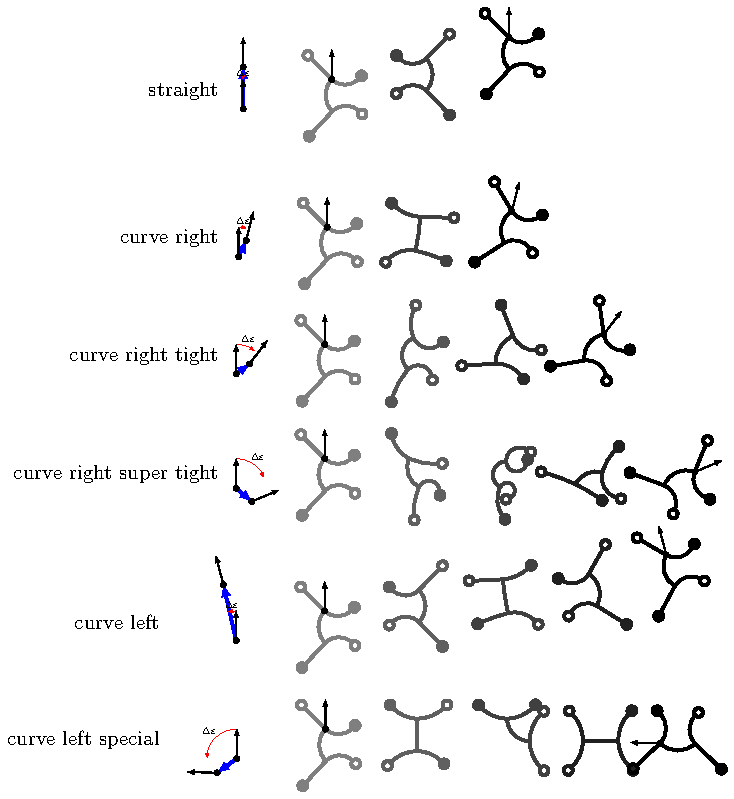
\includegraphics[width=.95\textwidth]{pics/trajectory_planner/elements.pdf}

\begin{itemize}
	\item Idee: Eine ausgewählte Anzahl an Posen, als Grundbausteine für einen beliebigen Gang.
	
	\item Diese dann wie Legosteine aufeinander setzen, um von A nach B zu gelangen.
\end{itemize}


\subsection{Search Tree}

\begin{itemize}
	\item Folgender Suchbaum wurde implementiert.
\end{itemize}

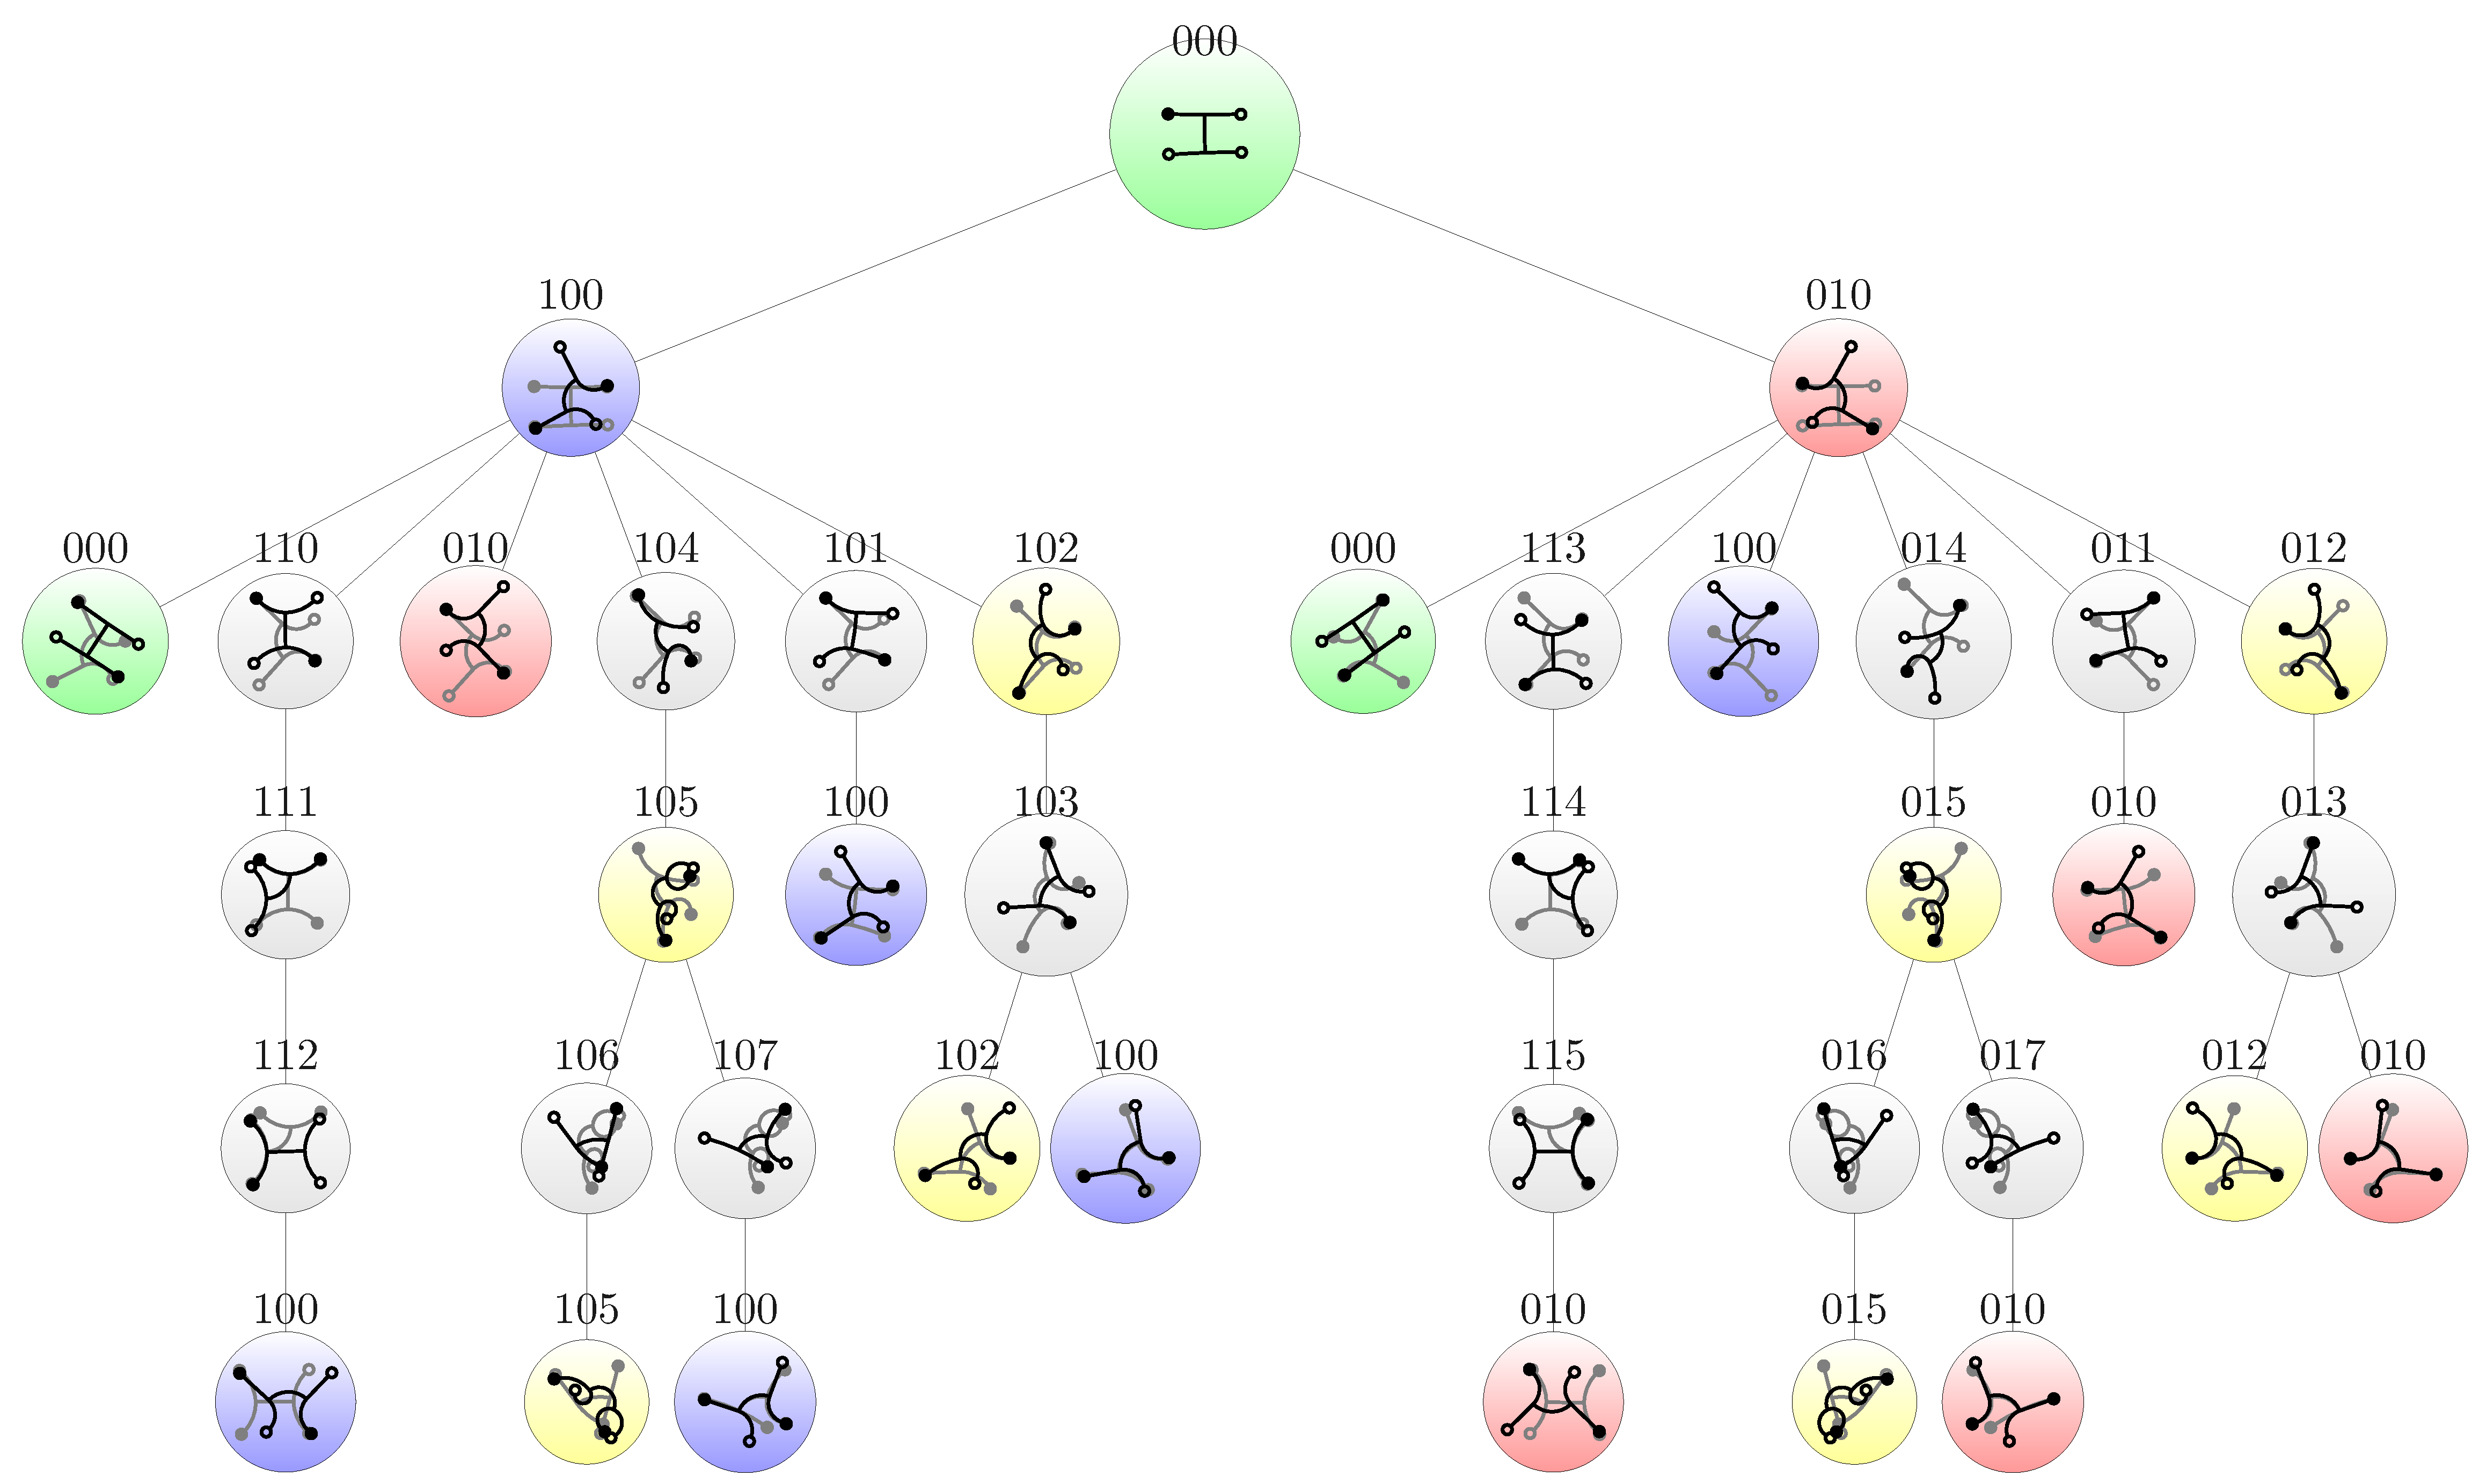
\includegraphics[width=.99\textwidth]{pics/trajectory_planner/tree.pdf}

\begin{tabular}{r|l}

\tikz\node[fill=green]{Green}; & Ruhe Pose \\
\tikz\node[fill=blue]{Blue}; & Rechte Adapter Pose\\
\tikz\node[fill=red]{Red}; & Linke Adapter Pose\\
\tikz\node[fill=yellow]{Yellow}; & Zwischen-Adapterpose für Kurven Looping\\
\tikz\node[fill=gray]{Gray}; & Zwischenpose \\

\end{tabular}

\begin{itemize}
	\item Dabei hat jede Kante des Baums eine Richtung und eine Gewichtung $w$.

	\item Die Gewichtung $w = ((\delta x, \delta y), \delta \varepsilon)$ gibt an, inwieweit das entsprechende Kind (Folgepose repräsentiert durch den Knoten, der mit der gewichteten Kante mit dem momentanen Knoten $k$ verbunden ist) den Roboter relativ zur momentanen Orientierung bewegt: $(\delta x, \delta y)$ und wie weit diese Pose ihn drehen wird: $\delta \varepsilon$.

	\item Für eine gegebene, momentane Pose $\bm{\rho}_k$ wird für alle Kandidaten $j \in [0,\cdots,J-1]$ ausgerechnet, wieweit der Abstand $d_j$ der potentiell neuen Pose $\bm{\rho}_j$ zum Ziel $\bar{\bm{x}}$ ist:

	\begin{equation}
	d(\bm{\rho}_k, w_j, \bar{\bm{x}}) = \bigg| \bar{\bm{x}} - \left(\bm{p}_{1,k} + \bm{R}(\varepsilon_k)\begin{bmatrix}
	\delta x \\ \delta y
\end{bmatrix}	 \right)\bigg|_2
	\end{equation}	
	
	\item Außerdem wird die Richtungsabweichung $\Delta \varepsilon_j$ aller potentiell neuen Pose $j$ berechnet:
	
	\begin{equation}
	\Delta \varepsilon (\bm{\rho}_k, w_j, \bar{\bm{x}}) = \measuredangle\left( \bar{\bm{x}} - \left(\bm{p}_{1,k} + \bm{R}(\varepsilon_k)\begin{bmatrix}
	\delta x \\ \delta y
\end{bmatrix} \right), \bm{R}(\varepsilon_k + \delta \varepsilon) \begin{bmatrix}
1 \\ 0
\end{bmatrix} \right)
	\end{equation}

	\item Die Folgepose $\bm{\rho}_{k+1}$ ergibt sich dann aus dem Minimum der mit $a=.5$ gewichteten Summe von Abstand und Orientierungsabweichung für alle Möglichkeiten $\bm{\rho}_{j}$:
	
	\begin{equation}
	\bm{\rho}_{k+1} = \min_j \left( a \frac{d_j}{d_{\textnormal{min}}}  + (a-1)\frac{\Delta \varepsilon_j}{\Delta \varepsilon_{\textnormal{max}}} \right)
	\end{equation}

	\item wobei $\Delta \varepsilon_{\textnormal{max}}$ die maximale Orientierungsabweichung aller Möglichkeiten ist; und $d_{\textnormal{min}}$ der minimale Abstand aller Möglichkeiten ist.

\end{itemize}


\subsubsection{Search Tree with weights}
Complete SearchTree contains:

\begin{itemize}
	\item all vertices (i.e. poses) including fix and defix poses
	\item weights of egdes: $w = ((\delta x, \delta y), \delta \varepsilon)$
\end{itemize}

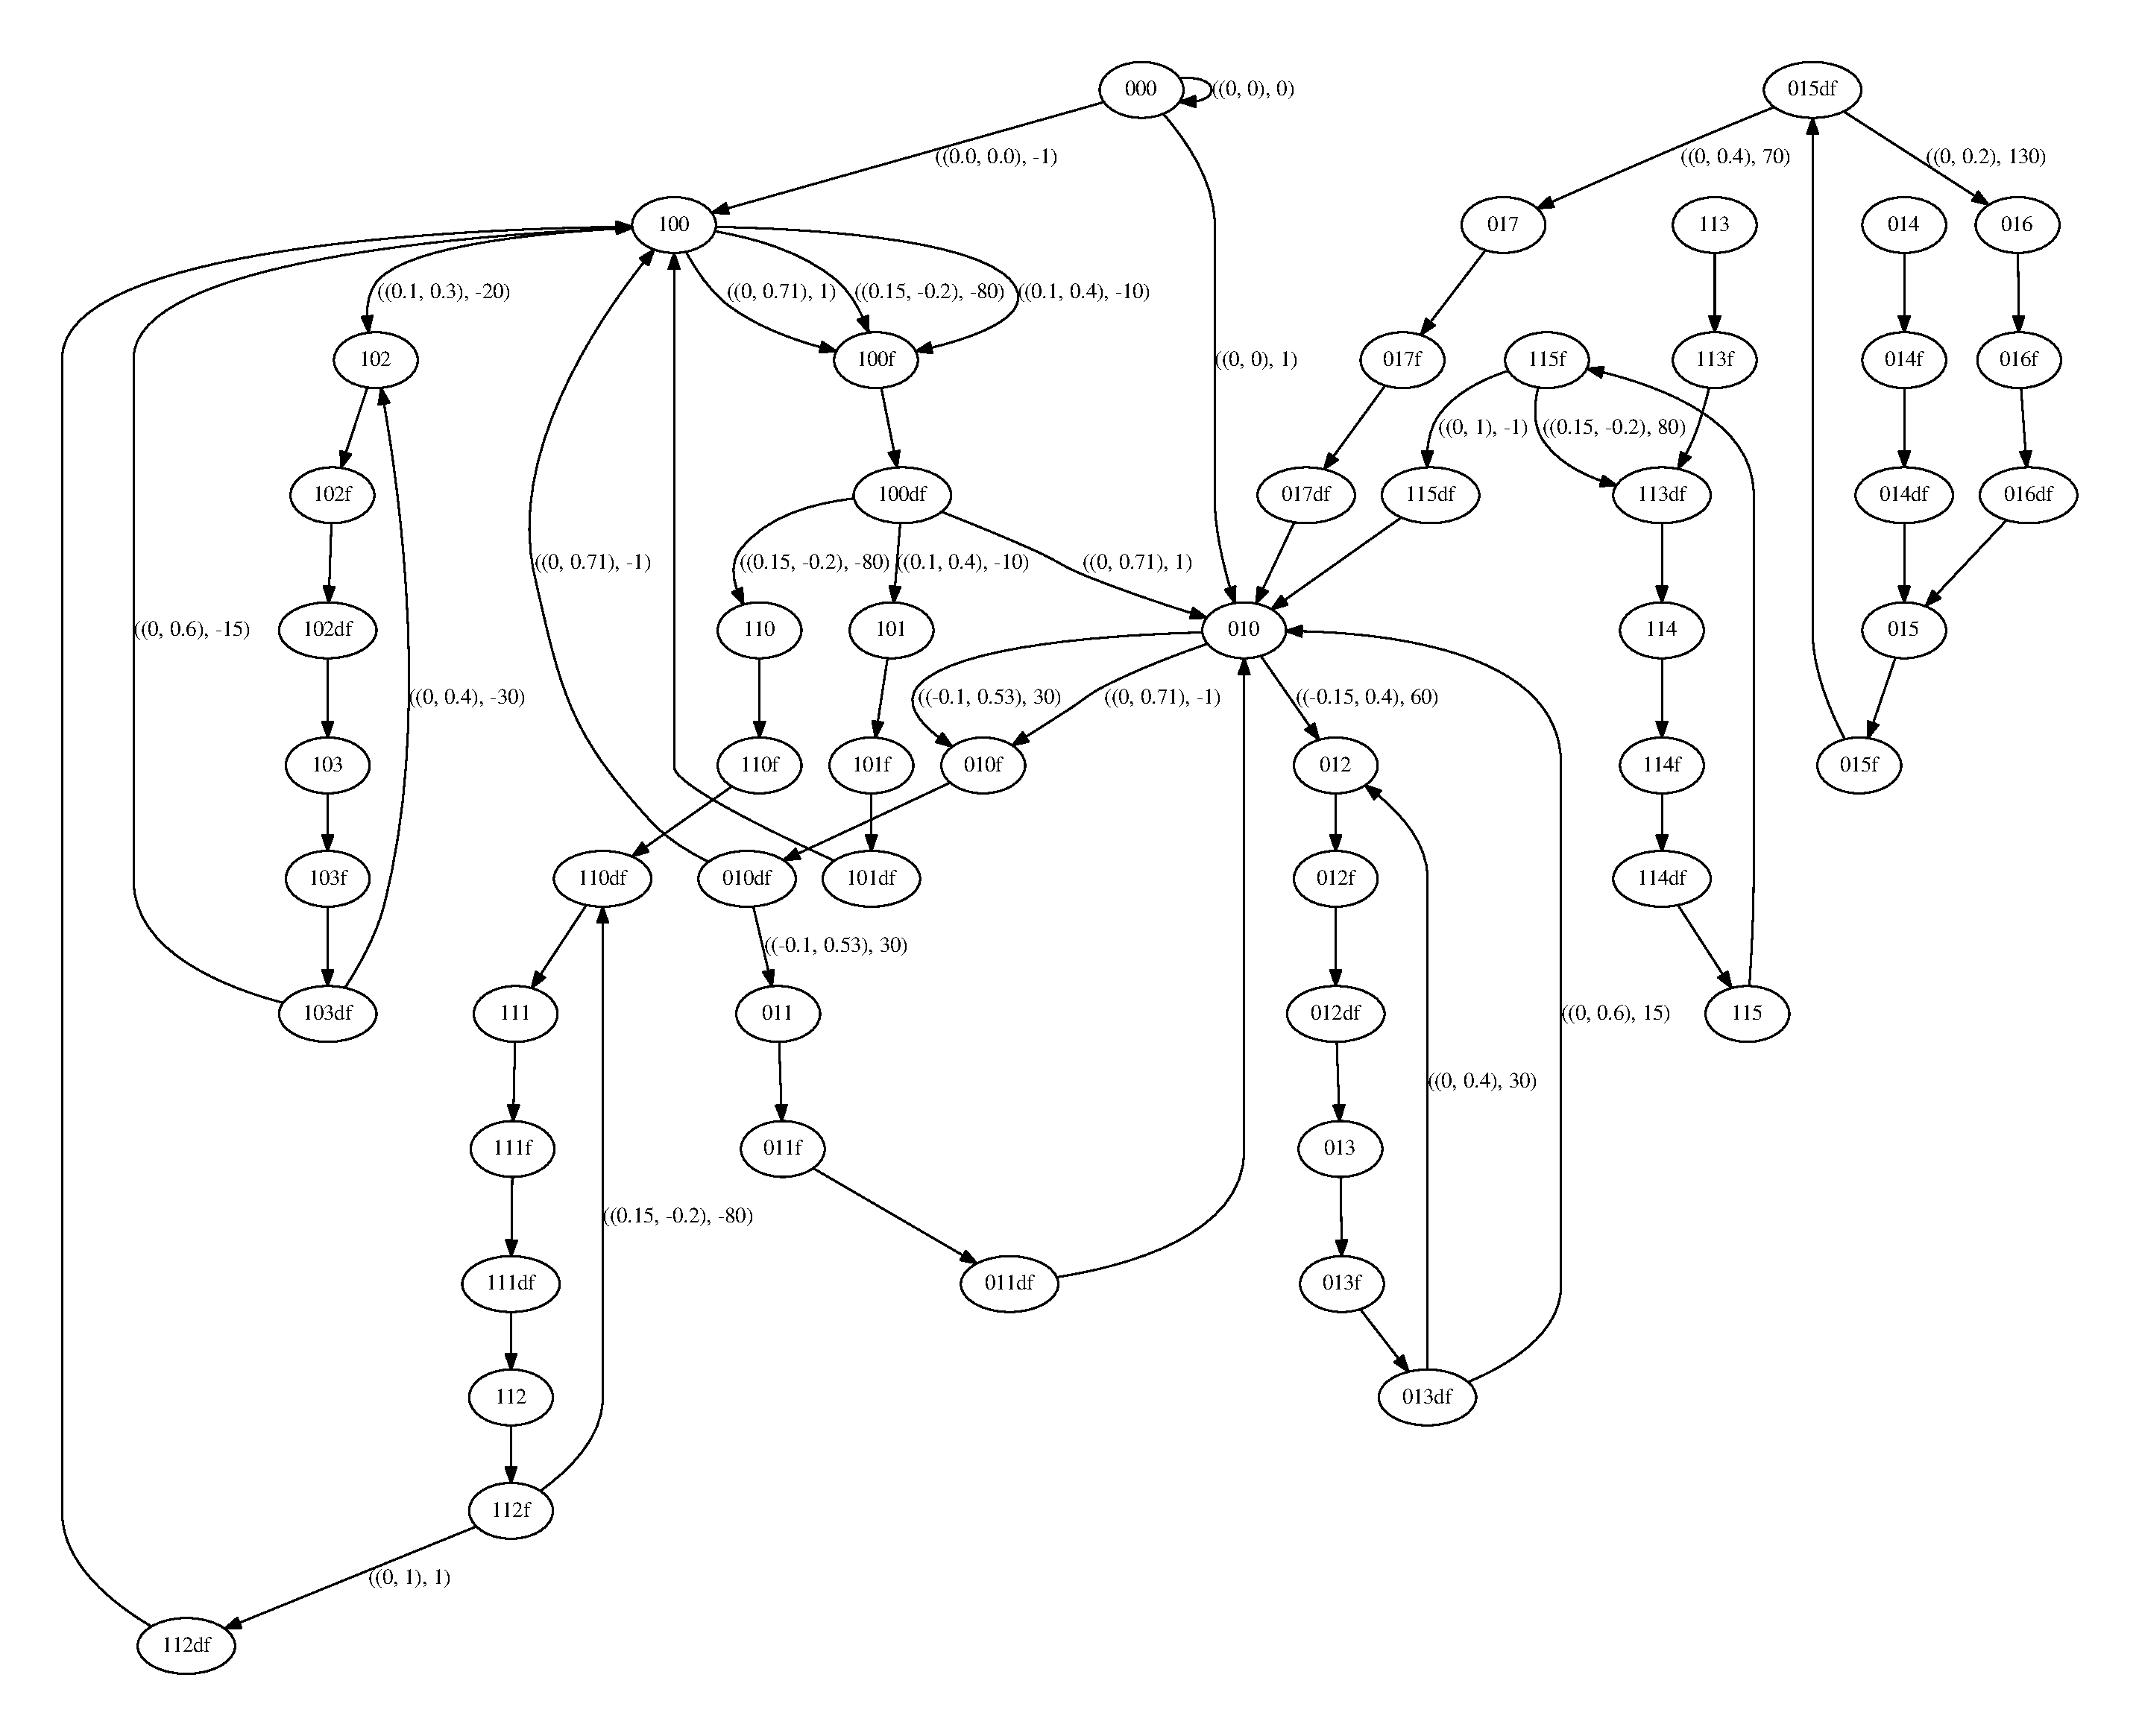
\includegraphics[width=.95\textwidth]{pics/trajectory_planner/tree_detail.pdf}


\subsection{Simulation Results}

Block Diagram of Simulation:

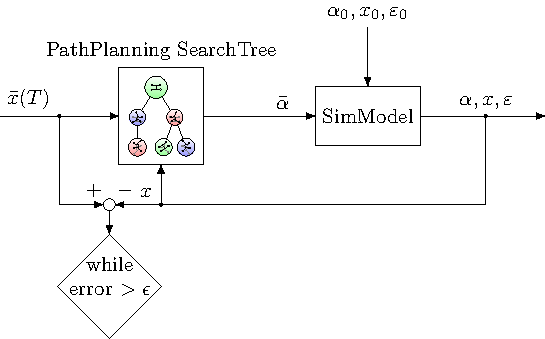
\includegraphics[scale=1]{pics/CtrLoops/pathplanner_searchtree.pdf}


\subsubsection{Simulation Results Curve}

\begin{itemize}
	\item Src: \texttt{path\_planner.py}
	
	\item Startwerte: $p_{1,0} = (0,0)$, $\bar{x} = (2,3)$, $\varepsilon_0 = 0$, $\alpha_0 = [90,0,-90,90,0]$
	
	\item Zu sehen sind:
	\begin{itemize}
		\item Der gesamte Gang
		\item Und alle Schritte, in denen eine Entscheidung getroffen werden musste.
		\item Die Position des Roboters und die Zielposition sind als rote Punkte markiert
		\item Das möglichen Folgeposen sind als orange Punkte dargestellt.
		\item Alle Orientierungen sind als blaue Linien dargestellt
	\end{itemize}

\end{itemize}


\begin{tabular}{ccc}
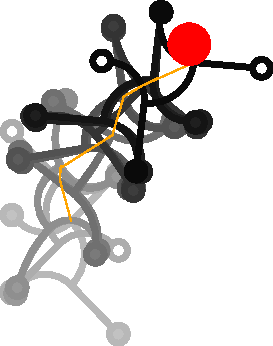
\includegraphics[scale=.8]{pics/pathplanner_without_noise/example_curve/gait.pdf}
&
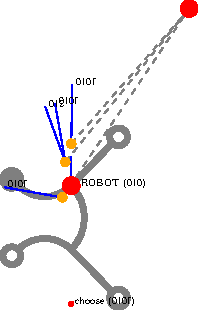
\includegraphics[scale=.8]{pics/pathplanner_without_noise/example_curve/dec_0.pdf}
&
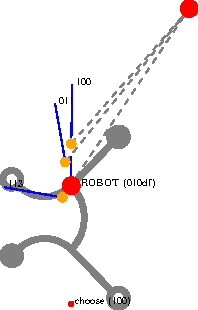
\includegraphics[scale=.8]{pics/pathplanner_without_noise/example_curve/dec_2.pdf}
\\
(a) & (b) & (c)
\\
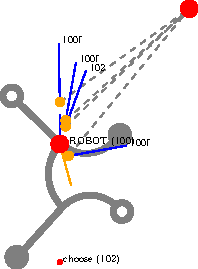
\includegraphics[scale=.8]{pics/pathplanner_without_noise/example_curve/dec_3.pdf}
&
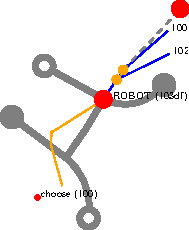
\includegraphics[scale=.8]{pics/pathplanner_without_noise/example_curve/dec_9.pdf}
&
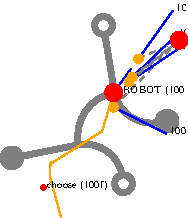
\includegraphics[scale=.8]{pics/pathplanner_without_noise/example_curve/dec_10.pdf}
\\
(d) & (e) & (f) 
\\
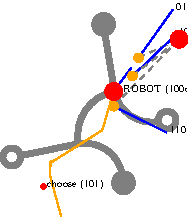
\includegraphics[scale=.8]{pics/pathplanner_without_noise/example_curve/dec_12.pdf}
&
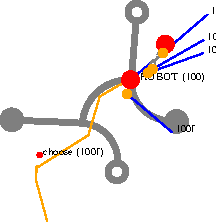
\includegraphics[scale=.8]{pics/pathplanner_without_noise/example_curve/dec_16.pdf}
&
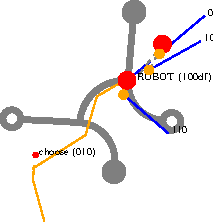
\includegraphics[scale=.8]{pics/pathplanner_without_noise/example_curve/dec_18.pdf}
\\
(g) & (h) & (i)\\
\end{tabular}

\subsubsection{Simulation Results Straight}

\begin{itemize}
	\item Src: \texttt{path\_planner.py}
	
	\item Startwerte: $p_{1,0} = (0,0)$, $\bar{x} = (2,13)$, $\varepsilon_0 = 0$, $\alpha_0 = [90,0,-90,90,0]$

\end{itemize}

\begin{tabular}{ccccc}
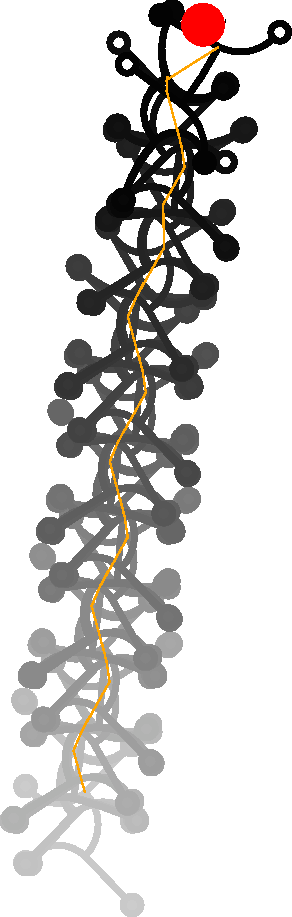
\includegraphics[scale=.8]{pics/pathplanner_without_noise/example_straight/gait.pdf}
&
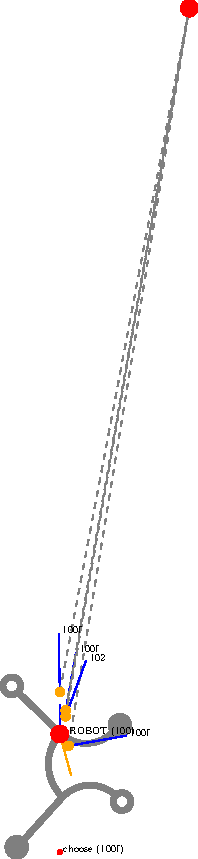
\includegraphics[scale=.8]{pics/pathplanner_without_noise/example_straight/dec_3.pdf}
&
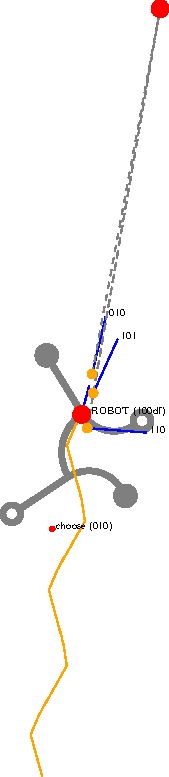
\includegraphics[scale=.8]{pics/pathplanner_without_noise/example_straight/dec_47.pdf}
&
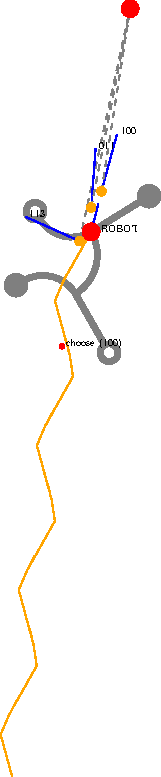
\includegraphics[scale=.8]{pics/pathplanner_without_noise/example_straight/dec_68.pdf}
&
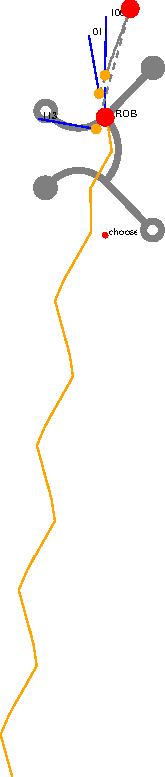
\includegraphics[scale=.8]{pics/pathplanner_without_noise/example_straight/dec_80.pdf}
\\
(a) & (b) & (c) & (d) & (e) 
\\
\end{tabular}



\subsection{What happens if Process Noise occurs?}

\begin{itemize}

	\item Es kann nicht davon ausgegangen werden, dass der Roboter stets exakt die ReferenzWinkel einnimmt.
	
	\item Diese Abweichung soll nun modelliert werden

	\item Add process noise to Simulation input (0 mean, 5 standard deviation)
	
	\item Implementierung: \texttt{alp = alp + np.random.normal(0, 5, 5)}

\end{itemize}

Block Diagram of Simulation with noise:

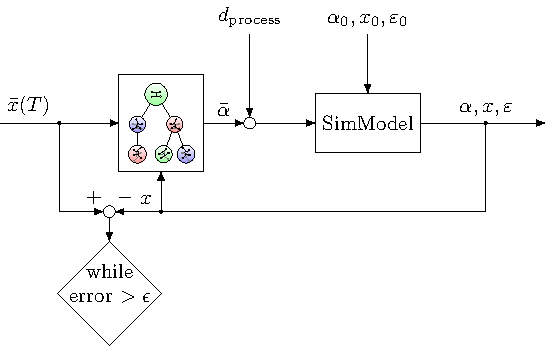
\includegraphics[scale=1]{pics/CtrLoops/pathplanner_searchtree_noise.pdf}

\subsubsection{Curve Noise}


\begin{itemize}
	\item Src: \texttt{path\_planner.py}
	
	\item Startwerte: $p_{1,0} = (0,0)$, $\bar{x} = (2,3)$, $\varepsilon_0 = 0$, $\alpha_0 = [90,0,-90,90,0]$
	
	\item Die Simulation wurde 5 mal wiederholt.
	
	\item Gezeigt ist jeweils nur der gesamte Gang.

\end{itemize}

\begin{tabular}{ccccc}
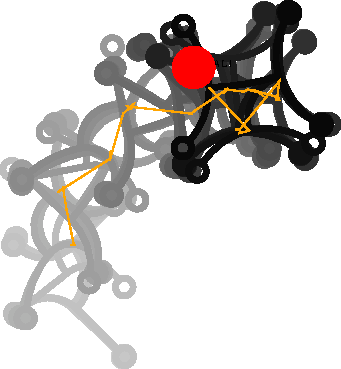
\includegraphics[scale=.5]{pics/pathplanner_with_noise/example_curve_01/gait.pdf}
&
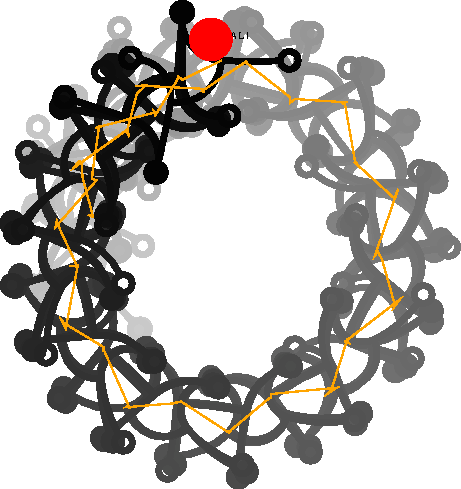
\includegraphics[scale=.5]{pics/pathplanner_with_noise/example_curve_02/gait.pdf}
&
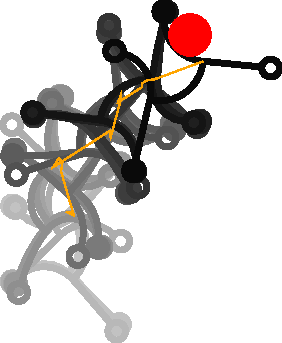
\includegraphics[scale=.5]{pics/pathplanner_with_noise/example_curve_03/gait.pdf}
&
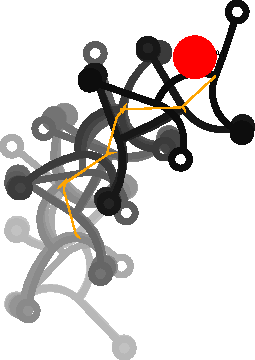
\includegraphics[scale=.5]{pics/pathplanner_with_noise/example_curve_04/gait.pdf}
&
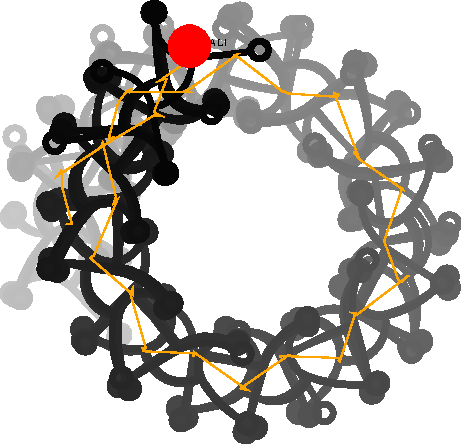
\includegraphics[scale=.5]{pics/pathplanner_with_noise/example_curve_05/gait.pdf}
\\
(a) & (b) & (c) & (d) & (e) 
\\
\end{tabular}

\subsubsection{Straight Noise}

\begin{itemize}
	\item Src: \texttt{path\_planner.py}
	
	\item Startwerte: $p_{1,0} = (0,0)$, $\bar{x} = (2,13)$, $\varepsilon_0 = 0$, $\alpha_0 = [90,0,-90,90,0]$
	
	\item Die Simulation wurde 5 mal wiederholt.
	
	\item Gezeigt ist jeweils nur der gesamte Gang.

\end{itemize}

\begin{tabular}{ccccc}
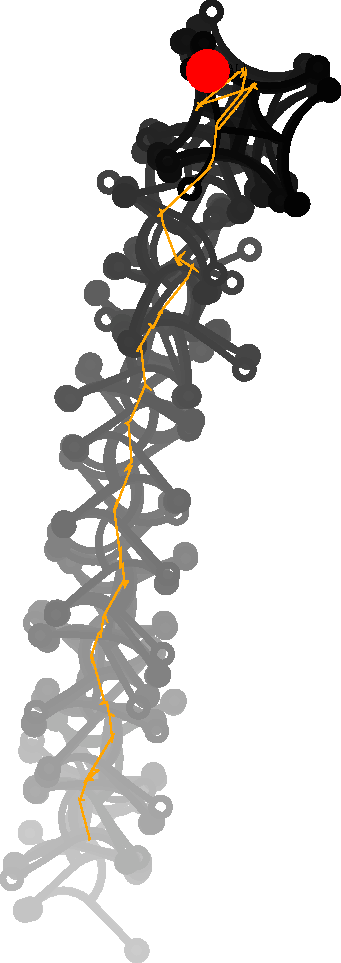
\includegraphics[scale=.5]{pics/pathplanner_with_noise/example_straight_01/gait.pdf}
&
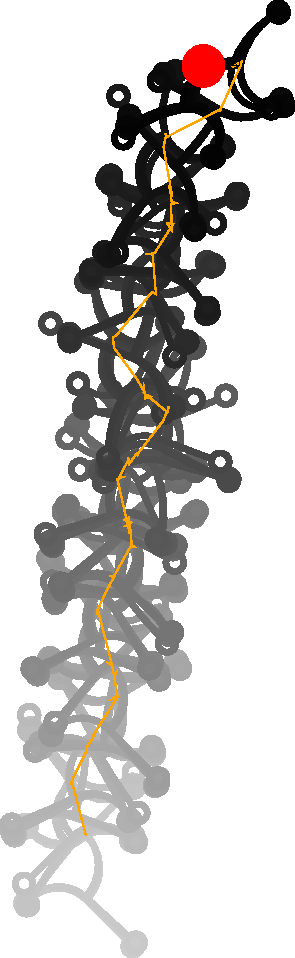
\includegraphics[scale=.5]{pics/pathplanner_with_noise/example_straight_02/gait.pdf}
&
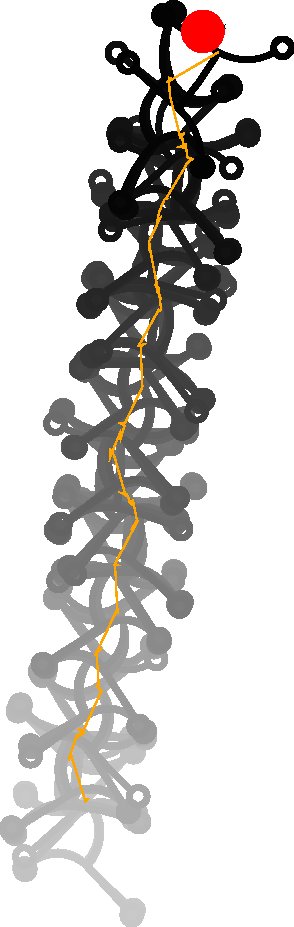
\includegraphics[scale=.5]{pics/pathplanner_with_noise/example_straight_03/gait.pdf}
&
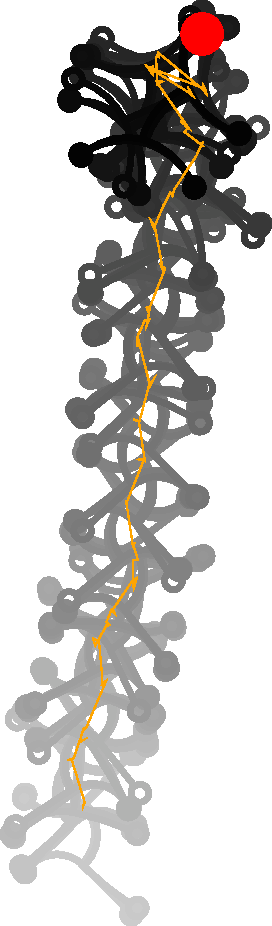
\includegraphics[scale=.5]{pics/pathplanner_with_noise/example_straight_04/gait.pdf}
&
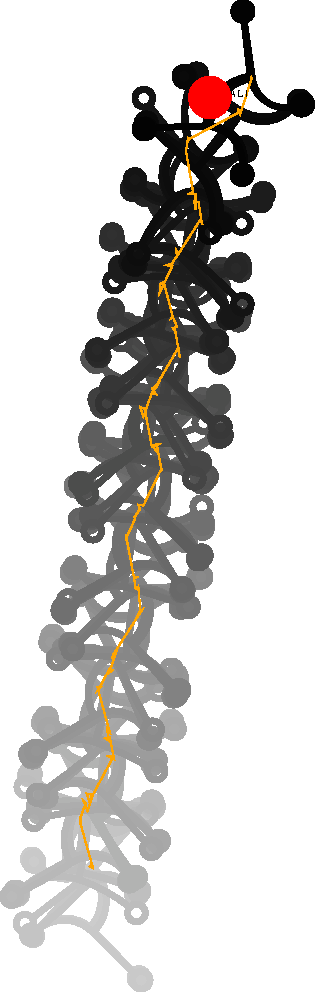
\includegraphics[scale=.5]{pics/pathplanner_with_noise/example_straight_05/gait.pdf}
\\
(a) & (b) & (c) & (d) & (e) 
\\
\end{tabular}



\subsection{Conclusion}

\begin{itemize}
	\item SearchTree Pathplanner funktioniert. Der Roboter kommt ans Ziel! Sowohl in der Simulation als auch im Experiment.
	\item Durch die finite Anzahl an möglichen Folgeposen, läuft der Roboter allerdings im ZickZack auf das Ziel zu.
	\item Wird Prozess Rauschen in die Simulation eingebaut, wird der Prozess instabil.
	\item Teilweise läuft der Roboter knapp am Ziel vorbei und ist in einem Kurven-Loop gefangen.
	\begin{itemize}
		\item Diese Phänomen konnte auch schon im Experiment gesichtet werden.
	\end{itemize}
	\item Fazit:
	\begin{itemize}
		\item PathPlanner SearchTree ist nicht wirklich flexibel. Kann zwar erweitert werden, aber umständlich.
		\item instabil bei ProzessRauschen.
	\end{itemize}	 
	
	

\end{itemize}




\section{Finding a Analytic Model for describing the General Gait}

\subsection{Problem Statement}

\begin{itemize}

\item Angenommen die Konfiguration / Pose des Roboters $\bm{\rho} = [\bm{\alpha}, \bm{p}_1, \varepsilon]$ ist vollständig bekannt, wobei $\bm{\alpha}$ die Gelenkkoordinaten / Biegewinkel der einzelnen Glieder sind, $\bm{p}_1$ die Position des vorderen Torsoendes und $\varepsilon$ die Orientierung des Roboters.
Siehe Bild:

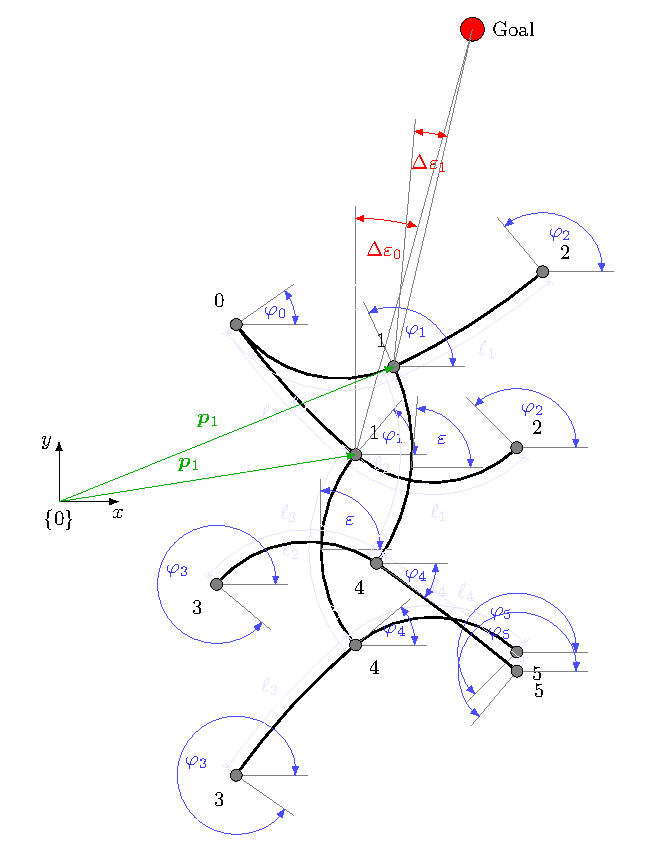
\includegraphics[width=8cm]{pics/general_model/model_vareps.pdf}


\item Für die Pfadplanung, wäre eine Funktion hilfreich, die zu einer gegebenen Wunschdrehung $\Delta \varepsilon$, eine entsprechende Abfolge von Roboter-Konfigurationen / Posen ausgibt, sodass sich der Roboter entsprechend dreht.

\item So könnte zB die Richtung des Roboters so justiert werden, dass er sich auf ein gegebenes Ziel zu bewegt.


\item Für den geraden Gang ist eine analytische Funktion bekannt, die die Geschwindigkeit des Roboters einstellt. Geschwindigkeit im Sinne von Schrittweite, bzw. Vorschub pro Zyklus:

\begin{equation}
\bm{\alpha} = \begin{bmatrix}
45 - \frac{x_1}{2} \\
45 + \frac{x_1}{2} \\
x_1 \\
45 - \frac{x_1}{2}  \\
45 + \frac{x_1}{2} \\
\end{bmatrix}
\end{equation}

Die Schrittweite ist hier als $x_1$ beschrieben.

\end{itemize}




\subsection{Approach: Guess structure for a analytic model for walking curves}

\begin{itemize}

\item Src can be found: \texttt{analytic\_model.py}

\item Model:

$x_1$ beschreibt hier die Schrittweite

$x_2$ das Maß der Drehung.

\begin{equation}
\bm{\alpha} = \begin{bmatrix}
45 - \frac{x_1}{2} \\
45 + \frac{x_1}{2} \\
x_1 + x_2 \\
45 - \frac{x_1}{2}  \\
45 + \frac{x_1}{2} \\
\end{bmatrix}
\end{equation}

\item Method:

Simulate for different $x_1$ and $x_2$ (in der Abbildung unten ist $x_1$ = \texttt{gam} und $x_2$ = \texttt{x})


\end{itemize}


\subsubsection{Simulation Results}

Results für 2 Zyklen:

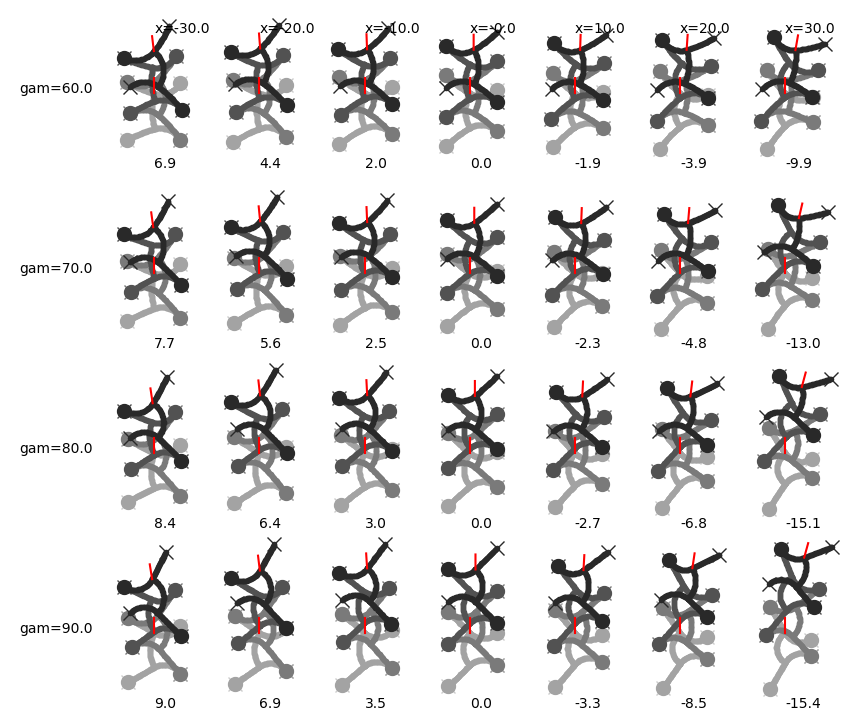
\includegraphics[width=12cm]{pics/model_1/GeckoBotGait_2cyc.png}


\subsubsection{Observations}

\begin{itemize}
	\item Es funktioniert. Der Roboter läuft eine Kurve.
	\item Kurve ist unsymmetrisch. Rechts klappt besser als links.
	\item Startpose ist besser für Rechtskurve geeignet.
	\item Noch nichts über die innere SPannung des Roboters herausgefunden
\end{itemize}




\subsection{Approach: Find a reasonable structure}

\begin{itemize}

\item Src can be found:

	\begin{tabular}{ll}
		 \texttt{analytic\_model\_2.py} & First Tries \\
		 \texttt{analytic\_model\_2\_adv.py} & Final Results \\
	\end{tabular}

\item Orientierung der Füße soll konstant bleiben:

\begin{equation}
\varphi_0 = \varepsilon + \frac{\alpha_2}{2} - \alpha_0
\end{equation}

Da im vorhergegangenem Versuch die asymmetrischen Aktuierung des Torsos schon zu guten Ergebnissen geführt hat, soll dieses Modell beibehalten werden. Allerdings in einer leicht variierten Form. $x_2$ ist nun ein relatives Maß für die Drehung:
\begin{equation}
\alpha_2 = x_1 + x_2|x_1|
\end{equation}


Es muss also $\alpha_0$ so gewählt werden, dass $\varphi_0$ möglichst unabhängig von $x_i$ wird.
Deshalb wird ein noch unbekannter Term $x_3$ hinzugefügt. Damit ergibt sich der Biegewinkel des Beines:

\begin{equation}
\alpha_0 = 45+ \frac{x_1}{2} + x_3.
\end{equation}

Für die Orientierung des Fußes bedeutet das:
\begin{eqnarray}
\varphi_0 &=& \varepsilon + \frac{x_1 + x_2|x_1|}{2} - \left( 45 + \frac{x_1}{2} + x_3 \right) \\
			&=& \varepsilon -45 + \frac{x_2|x_1|}{2} -x_3 \\
\end{eqnarray}

Es wird \textbf{angenommen}, dass die Orientierung des Roboters mit der Schrittweite linear wächst (i.e. Der Roboter dreht sich ein wenig zwischen seinen Extremposen):
\begin{equation}
\varepsilon = c_1 x_1 + \varepsilon_0
\end{equation}

Mit konstantem Orientierungswinkel $\varphi = \varphi_0$ ergibt sich somit:

\begin{eqnarray}
\varphi_0 &=& c_1 x_1 + \varepsilon_0 - 45 + \frac{x_2|x_1|}{2} -x_3 \\
x_3 &=&  c_1 x_1 + \frac{x_2|x_1|}{2} + c
\end{eqnarray}

Unter der \textbf{Annahme}, dass $\varphi_0 \approx \varepsilon_0 - 45$ ist, ergibt sich $c \approx 0$. Das meint, die Orientierung ändert sich nur minimal. entspricht also im Wesentlichen der Ausgangskonfiguration.
Weiterhin wird \textbf{angenommen}, dass für einen fixierter Fuß der Term $c_1x_1 \approx 0$ vernachlässigbar ist.
Somit ergibt sich für den Biegewinkel des fixierten vorderen linken Beins:

\begin{equation}
\alpha_{0,f} = 45-\frac{x_1}{2} + \frac{1}{2}x_2|x1|
\end{equation}

Wenn das Bein nicht fixiert ist, kann es beliebige Orientierung annehmen.
Hierfür wird \textbf{angenommen}, dass sich die Drehung des Körpers erst in der nicht fixierten Phase eines Beines in desses Orientierung auswirkt.
Deshalb, wird der Term $c_1x_1$ in dieser Phase aktiv.
Weiterhin wird \textbf{angenommen}, dass $c_1 = x_2$. Damit ergibt sich für einen nicht fixierten Fuß:

\begin{equation}
\alpha_{0,\bar{f}} = 45-\frac{x_1}{2} + x_2x1
\end{equation}


\item Das resultierende Modell sieht so aus:

\begin{equation}
\bm{\alpha} = \begin{bmatrix}
45 - \frac{x_1}{2}+ f_0\frac{1}{2}|x1|x_2  + \bar{f}_0x_1x_2  \\
45 + \frac{x_1}{2} + f_1\frac{1}{2}|x1|x_2+ \bar{f}_1x_1x_2  \\
x_1 + |x_1|x_2 \\
45 - \frac{x_1}{2}  + f_2\frac{1}{2}|x1|x_2 + \bar{f}_2x_1x_2\\
45 + \frac{x_1}{2}  + f_3\frac{1}{2}|x1|x_2+ \bar{f}_3x_1x_2 \\
\end{bmatrix}
\end{equation}

Wobei $f_i$ den Zustand des Fußes beschreibt:

\begin{equation}
f_i = \left[
\begin{matrix}
1 & if & \textnormal{foot fixed} \\ 
0 & else& \\
\end{matrix} \right.
\end{equation}
\begin{equation}
\bar{f}_i = \left[
\begin{matrix}
0 & if& \textnormal{foot fixed} \\ 
1 & else& \\
\end{matrix} \right.
\end{equation}
\end{itemize}

\subsubsection{Simulation Results}

\begin{itemize}
	\item In der abgebildeten Matrix sind in den Reihen konstante Schrittweite $x_1$ 
	\item Spalten: konstantes Kurvenmaß $x_2$
	\item Jedes Einzelbild zeigt die Simulation von zwei Zyklen mit dem zu $(x_1, x_2)$ entsprechenden Laufmuster.
	\item Unter jedem Einzelbild ist die Drehung in Grad $\Delta \varepsilon$ und die Summe der inneren Spannung aller Posen innerhalb des Laufes $\sum_i \sigma(\bm{\rho}_i)$.
	
\end{itemize}


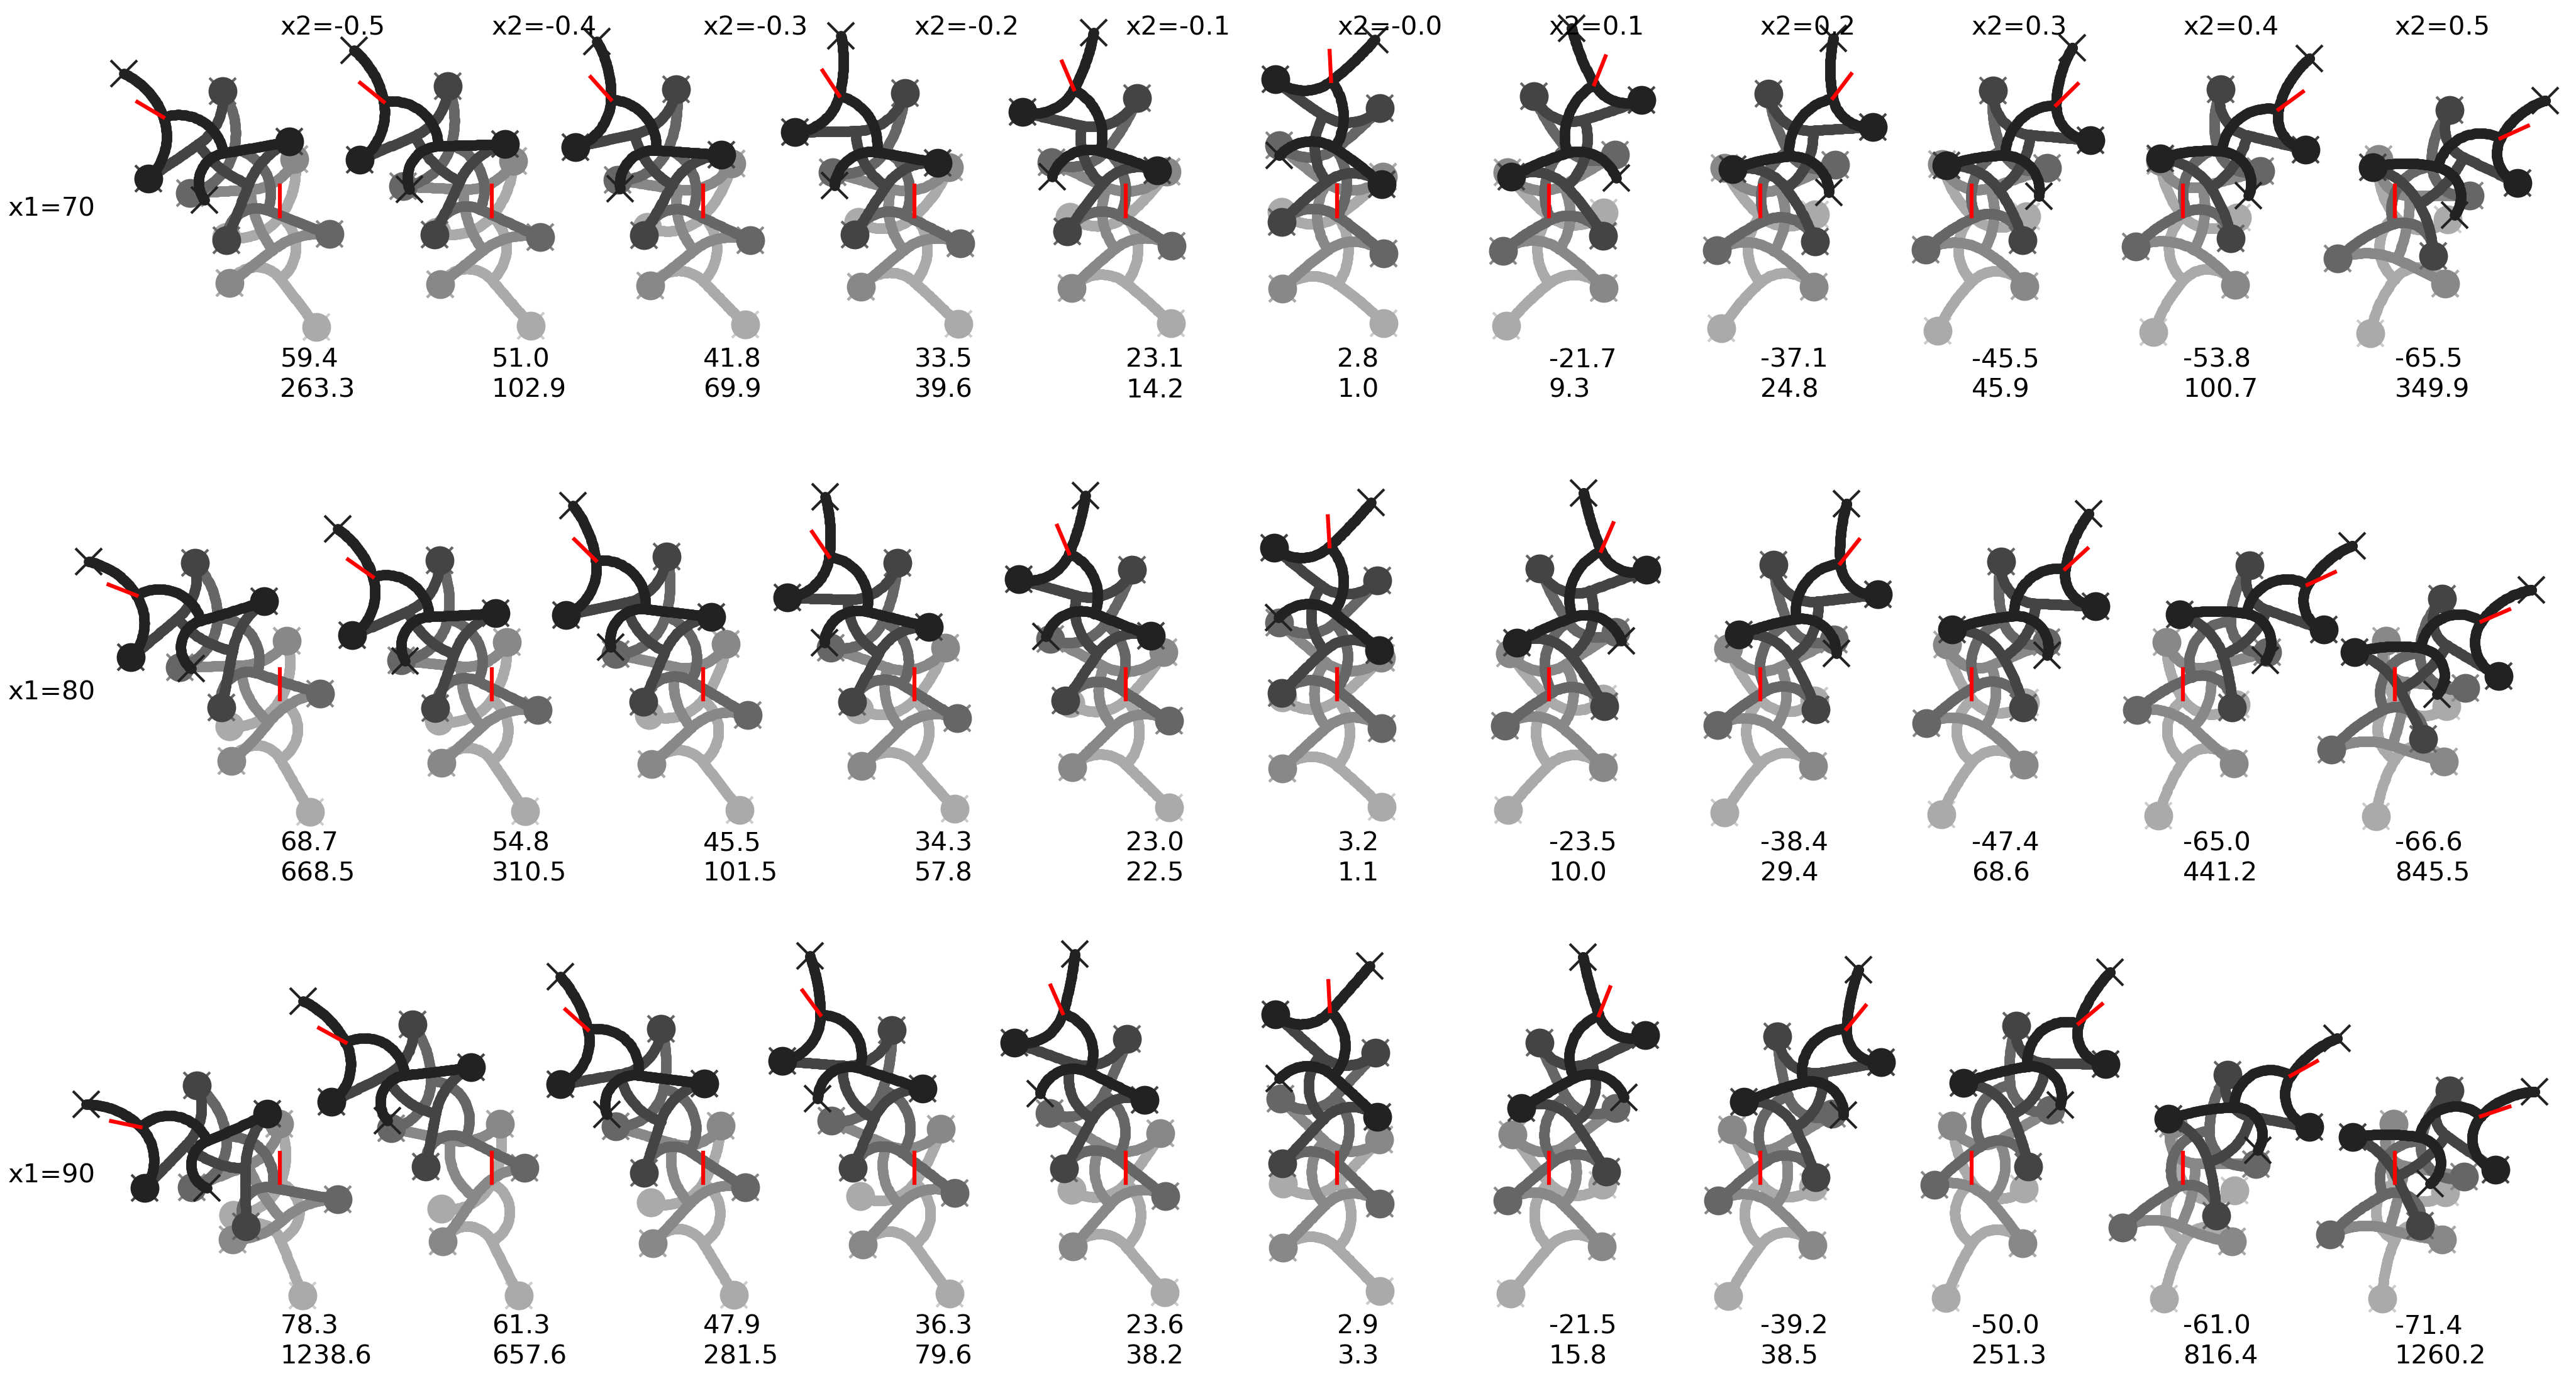
\includegraphics[width=.95\textwidth]{pics/model_2/gait.jpg}


\begin{itemize}
	\item Folgende Abbildung zeigt den Stressverlauf $\sigma(\bm{\rho}_i)$
	
	\item Bis auf ein paar Ausreißer ist die innere Spannung über den Lauf moderat.
\end{itemize}

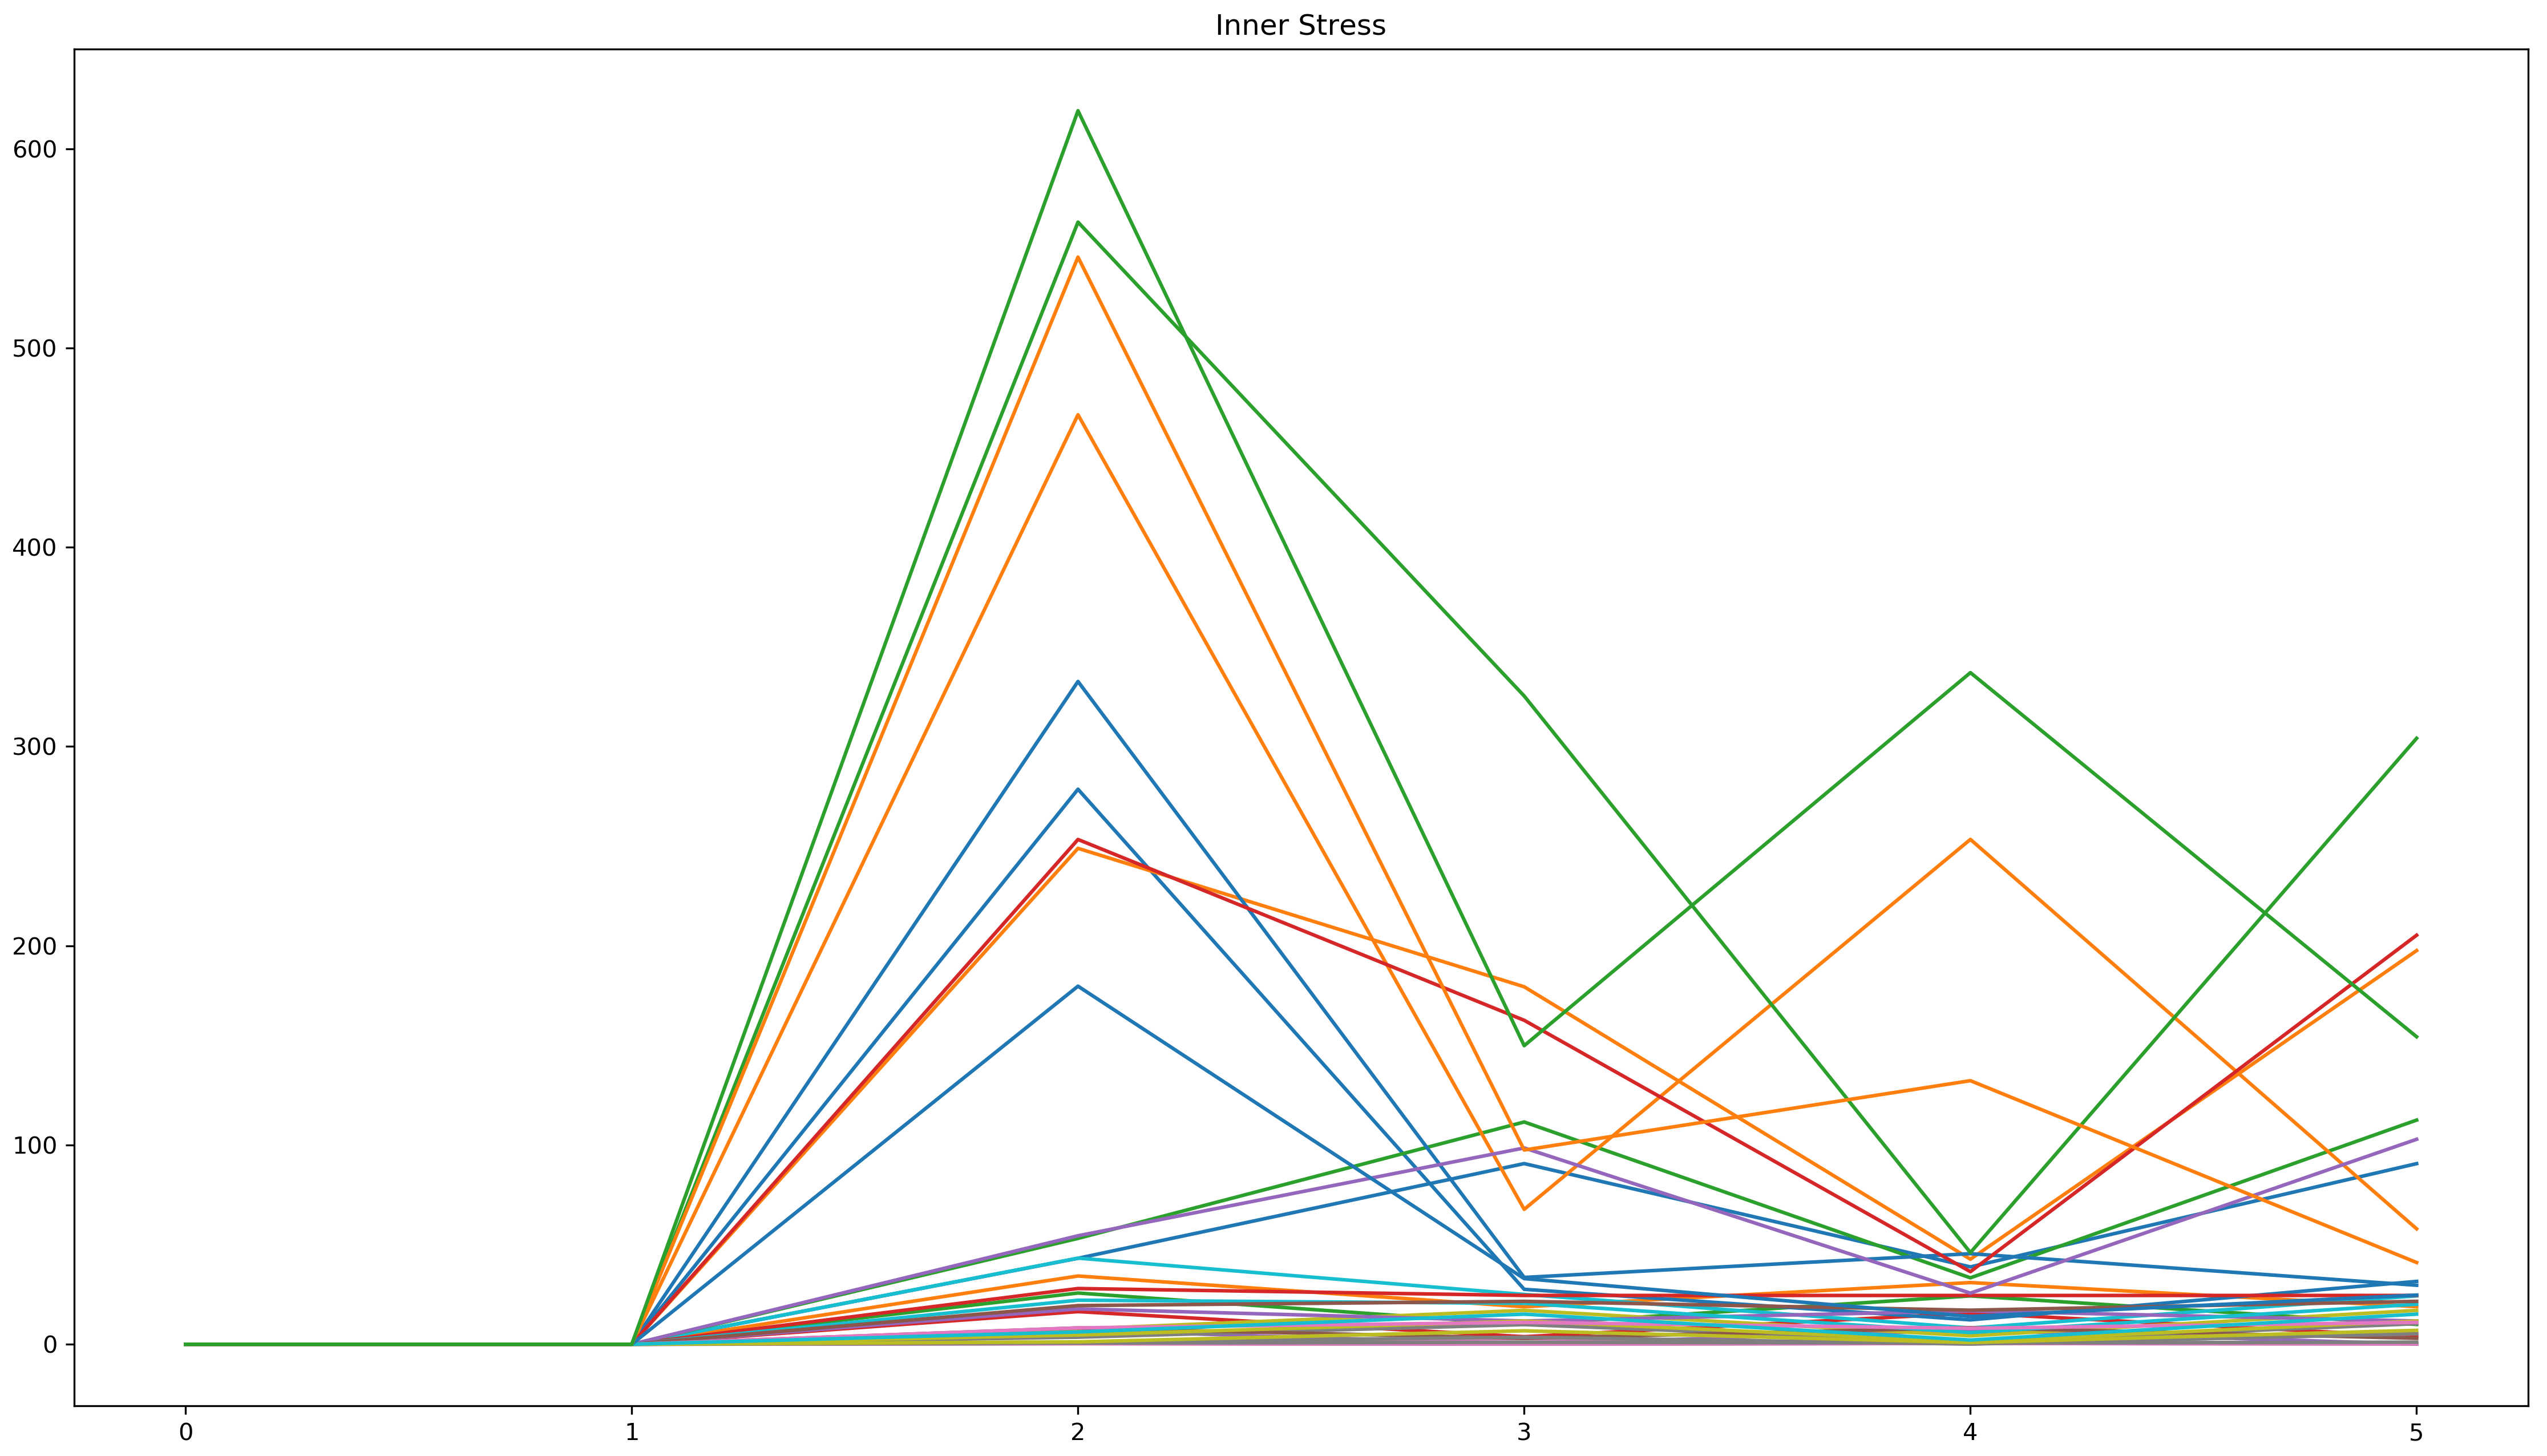
\includegraphics[width=.95\textwidth]{pics/model_2/GeckoBotGaitStress.jpg}


\begin{itemize}
	\item Delta Epsilon kann jetzt gefittet werden:
	
	\begin{equation}
	\frac{\Delta \varepsilon}{2 cycle} (x_1, x_2) = -21.7 x_2 -.51 x_2^2 - 1.67x_1x_2
	\end{equation}
	
	\item SurfacePlot ist Simulations Data und WirframPlot ist der Fit
\end{itemize}

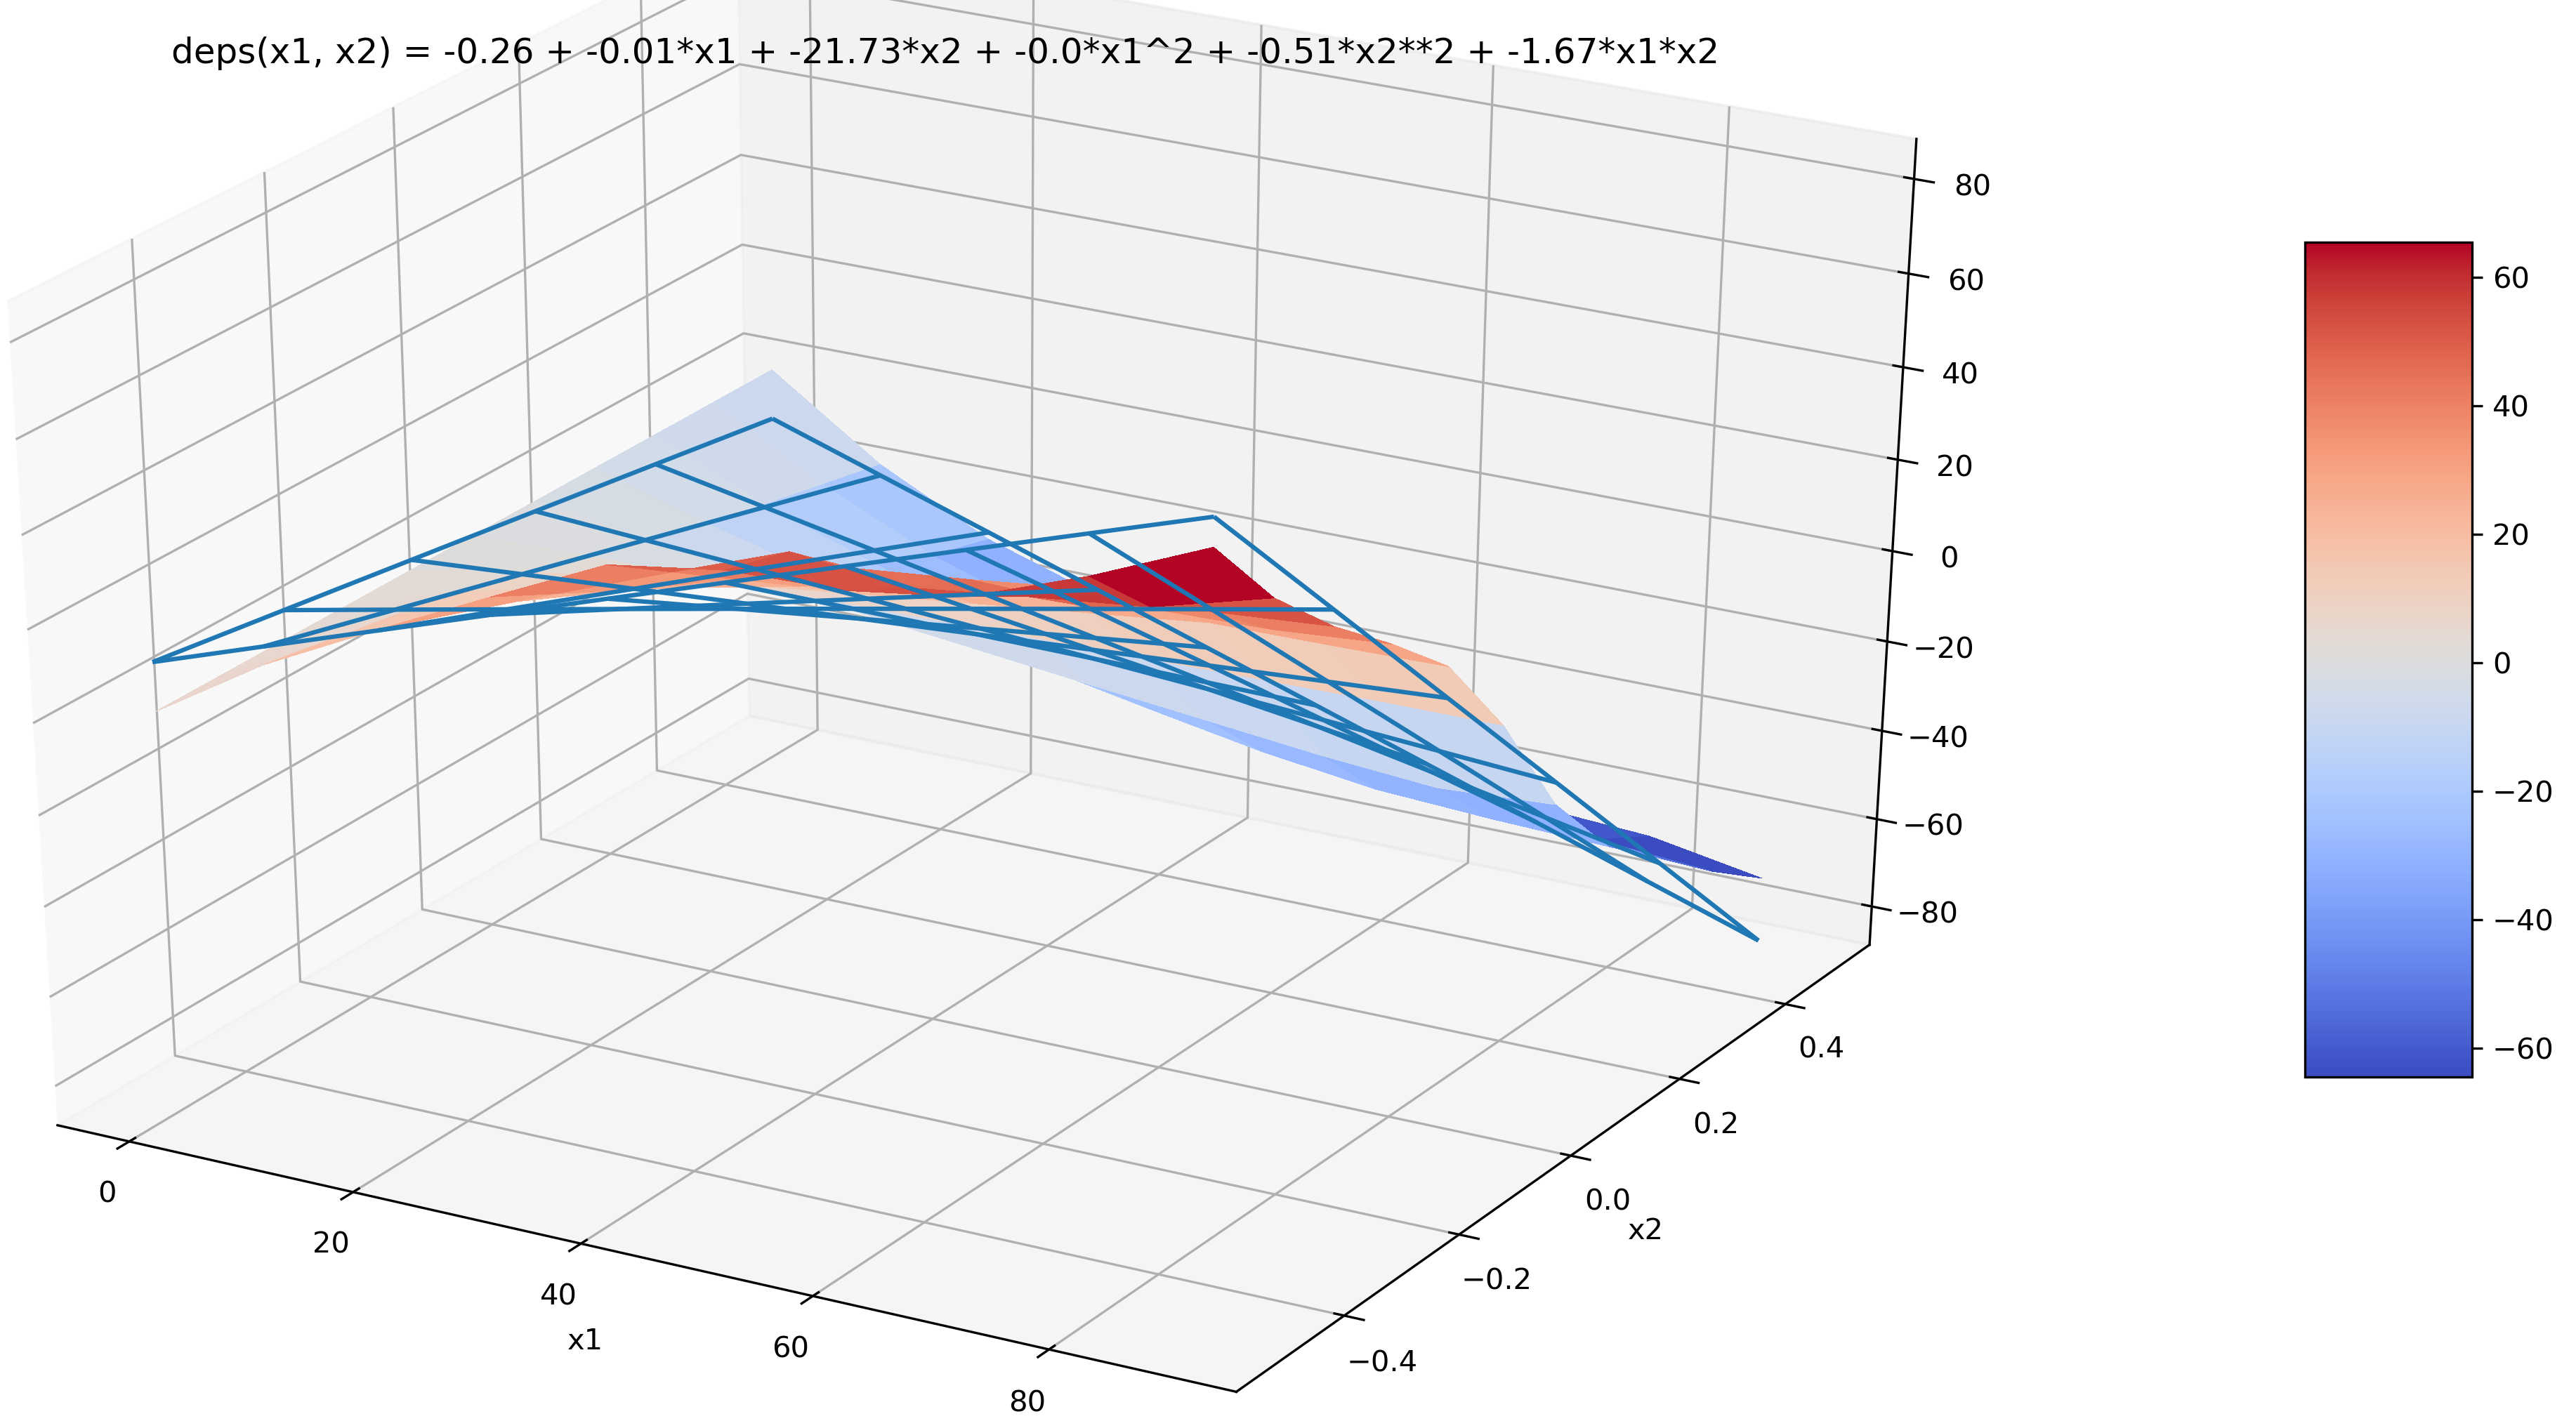
\includegraphics[width=.95\textwidth]{pics/model_2/Fit.jpg}

\begin{itemize}
	\item Ebenso kann die Translation in Bewegungsrichtung gefittet werden:
	\begin{equation}
		\frac{\begin{bmatrix}	\delta x \\ \delta y \end{bmatrix} (x_1, x_2)}{1 cycle} = \begin{bmatrix}
		.07x_2 - .29 x_2^2 + .02 x_1x_2 \\
		.02x_1 + .13x_2 - .47x_2^2 \\
		\end{bmatrix}
	\end{equation}
	\item Schwarze Pfeile sind Fit. Bunte Pfeile Simulations Ergebnisse.
\end{itemize}

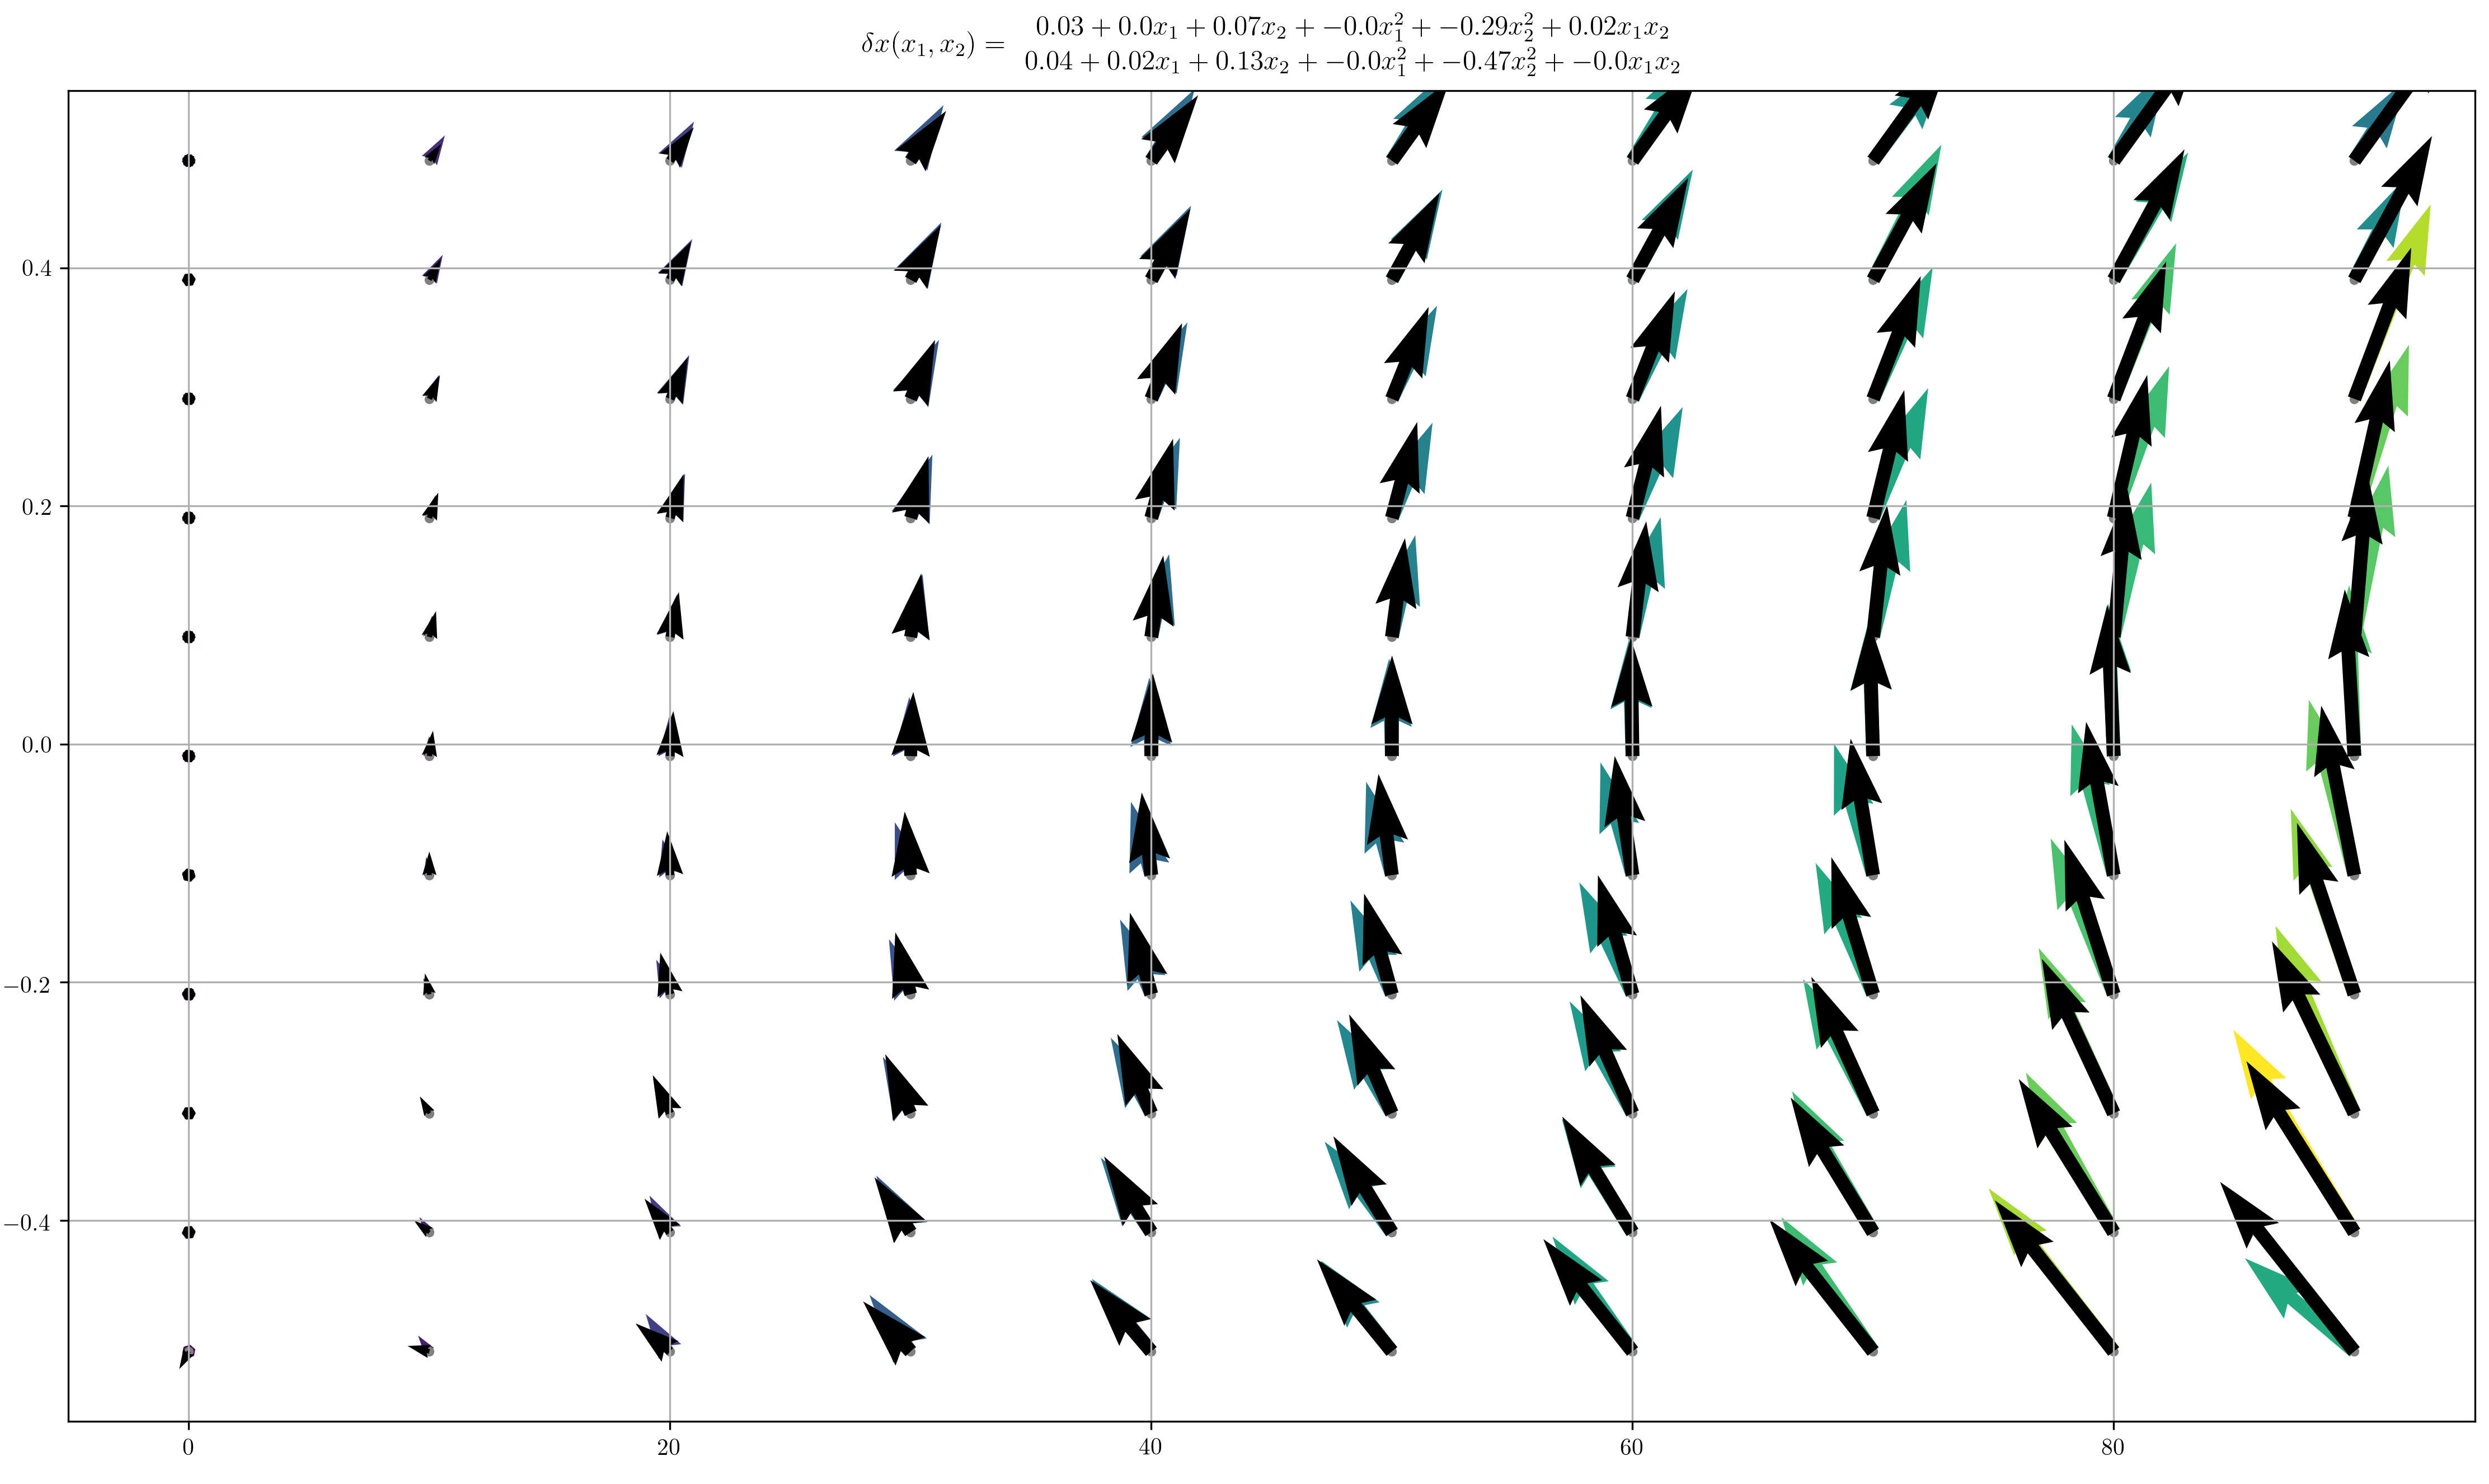
\includegraphics[width=.95\textwidth]{pics/model_2/FitDXDY_1cyc.jpg}



\subsection{Approach: Optimize Extra leg bending Angle for given extra torso bending}

\begin{itemize}

\item Src can be found: 

	\begin{tabular}{ll}
	\texttt{analytic\_model\_3.py} & Optimizing $x_3$ und $x_4$ \\
	\texttt{eval\_analytic\_model\_3.py} & Evaluate Simulation and Function Fitting  \\
	\texttt{eval2\_analytic\_model\_3.py} & Simulate Gait with obtained gait law \\
	\end{tabular}

\item Nun soll untersucht werden, welche Extra Leg Bending Angle die innere Spannung des Roboters minimiert.

\item Model:

\begin{equation}
\bm{\alpha} = \begin{bmatrix}
45 - \frac{x_1}{2} + \bar{f}_0x_3 + f_0x_4 \\
45 + \frac{x_1}{2} + \bar{f}_1x_3 + f_1x_4 \\
x_1|x_2| \\
45 - \frac{x_1}{2} + \bar{f}_2x_4 + f_3x_3 \\
45 + \frac{x_1}{2} + \bar{f}_3x_4 + f_4x_3 \\
\end{bmatrix}
\end{equation}


\item Annahme:

Die Extra Biegung $x_3$ für freie Beine und die Extra Biegung $x_4$ für fixierte Beine sind abhängig von der Extra Biegung $x_2$ für den Torso.

Hinter- und Vorderbeine sind nicht symmetrisch, aber kreuzweise symmetrisch:
Die Extrabiegung für ein \textbf{nicht fixiertes Vorderbein} entspricht der Extrabiegung eines \textbf{fixierten Hinterbeins} und anderesherum.


\item Methode:

Für gegebenes Extra Torso Bending $x_2$ und gegebenene Schrittweite $x1$ minimiere die Innere Spannung über den Gang mit $n$ Zyklen aufsummiert:

\begin{tabular}{c c l}
Gegeben: 	& $x_1$ & Schrittweite \\
			& $x_2$	& Extra Torsobiegung \\
Gesucht:	& $x_3$	& Extra Beinbiegung fixiert vorn \\
			& $x_4$	& Extra Beinbiegung fixiert hinten \\
\end{tabular}


\begin{equation}
 (x_{3,\textnormal{opt}}, x_{4,\textnormal{opt}}) = \min_{x_3, x_4} \sum_k^{2n} \sigma\Big(\bm{\rho}_k\big(\bm{\alpha}(x_1, x_2, x_3, x_4)\big)\Big)
\end{equation}

\end{itemize}


\subsubsection{Optimization Results}
Results (links mit Startwert (10, 20) rechts mit Startwert (20, 10)):

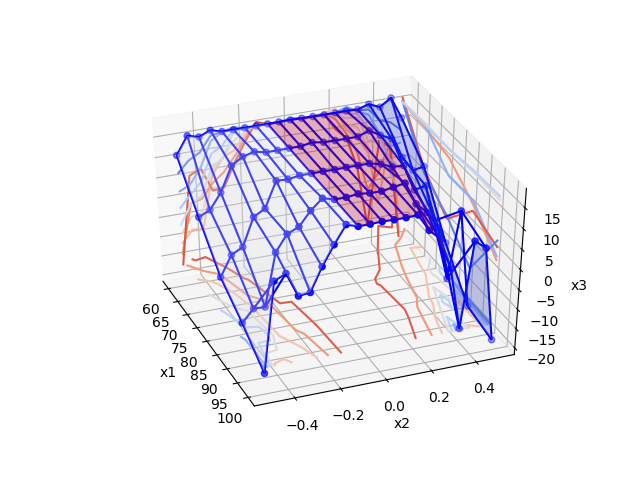
\includegraphics[width=.45\textwidth]{pics/model_3/X3-x0_0.png}
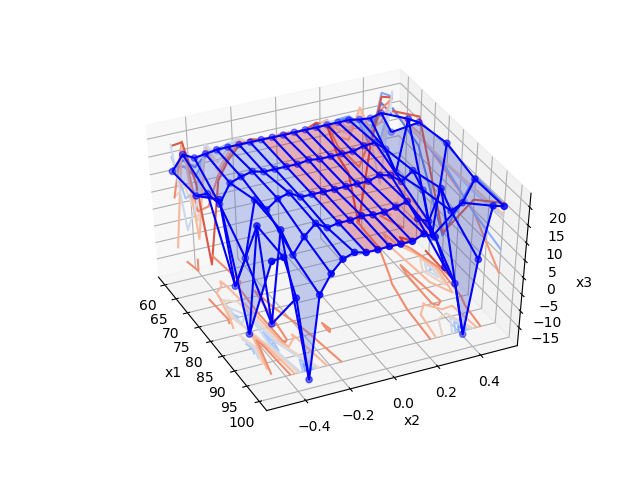
\includegraphics[width=.45\textwidth]{pics/model_3/X3-x0_1.png}

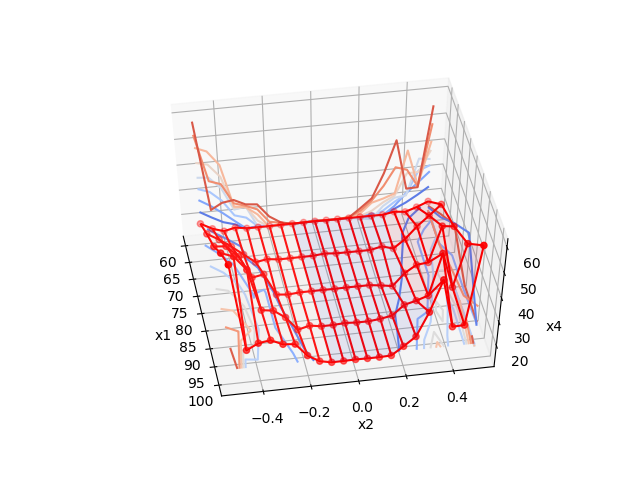
\includegraphics[width=.45\textwidth]{pics/model_3/X4-x0_0.png}
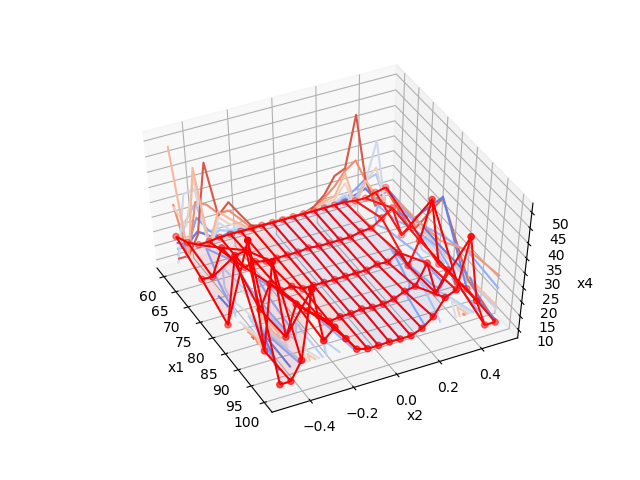
\includegraphics[width=.45\textwidth]{pics/model_3/X4-x0_1.png}

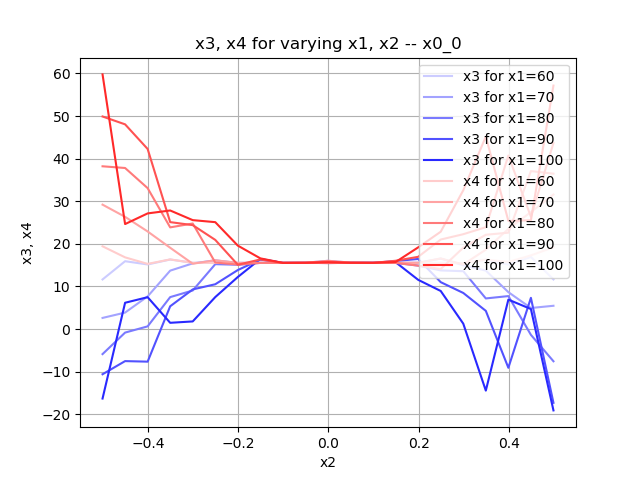
\includegraphics[width=.45\textwidth]{pics/model_3/X3-X4_-_x0_0_-_2D.png}
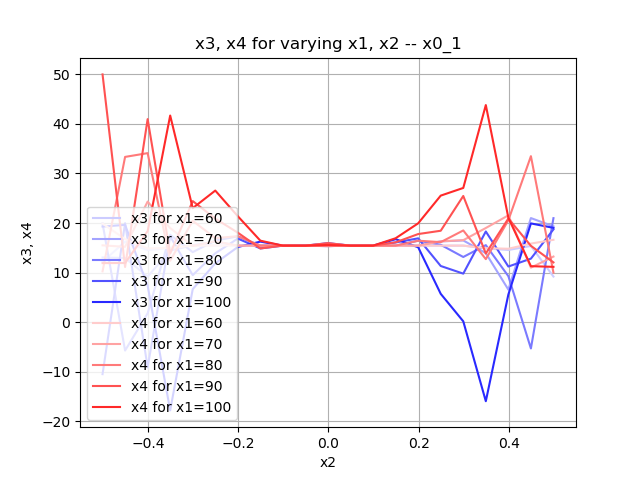
\includegraphics[width=.45\textwidth]{pics/model_3/X3-X4_-_x0_1_-_2D.png}


\subsubsection{Function Fitting}


\begin{itemize}
	\item Es werden Ergebnisse des ersten Startwert genommen.

	\item Es ergibt sich:
		\begin{equation}
		x_3 (x_1, x_2) = 30 - 2|x_1x_2| + 110|x_2|
		\end{equation}
		\begin{equation}
		x_4 (x_1, x_2) =  2|x_1x_2| - 80|x_2|
		\end{equation}
		
		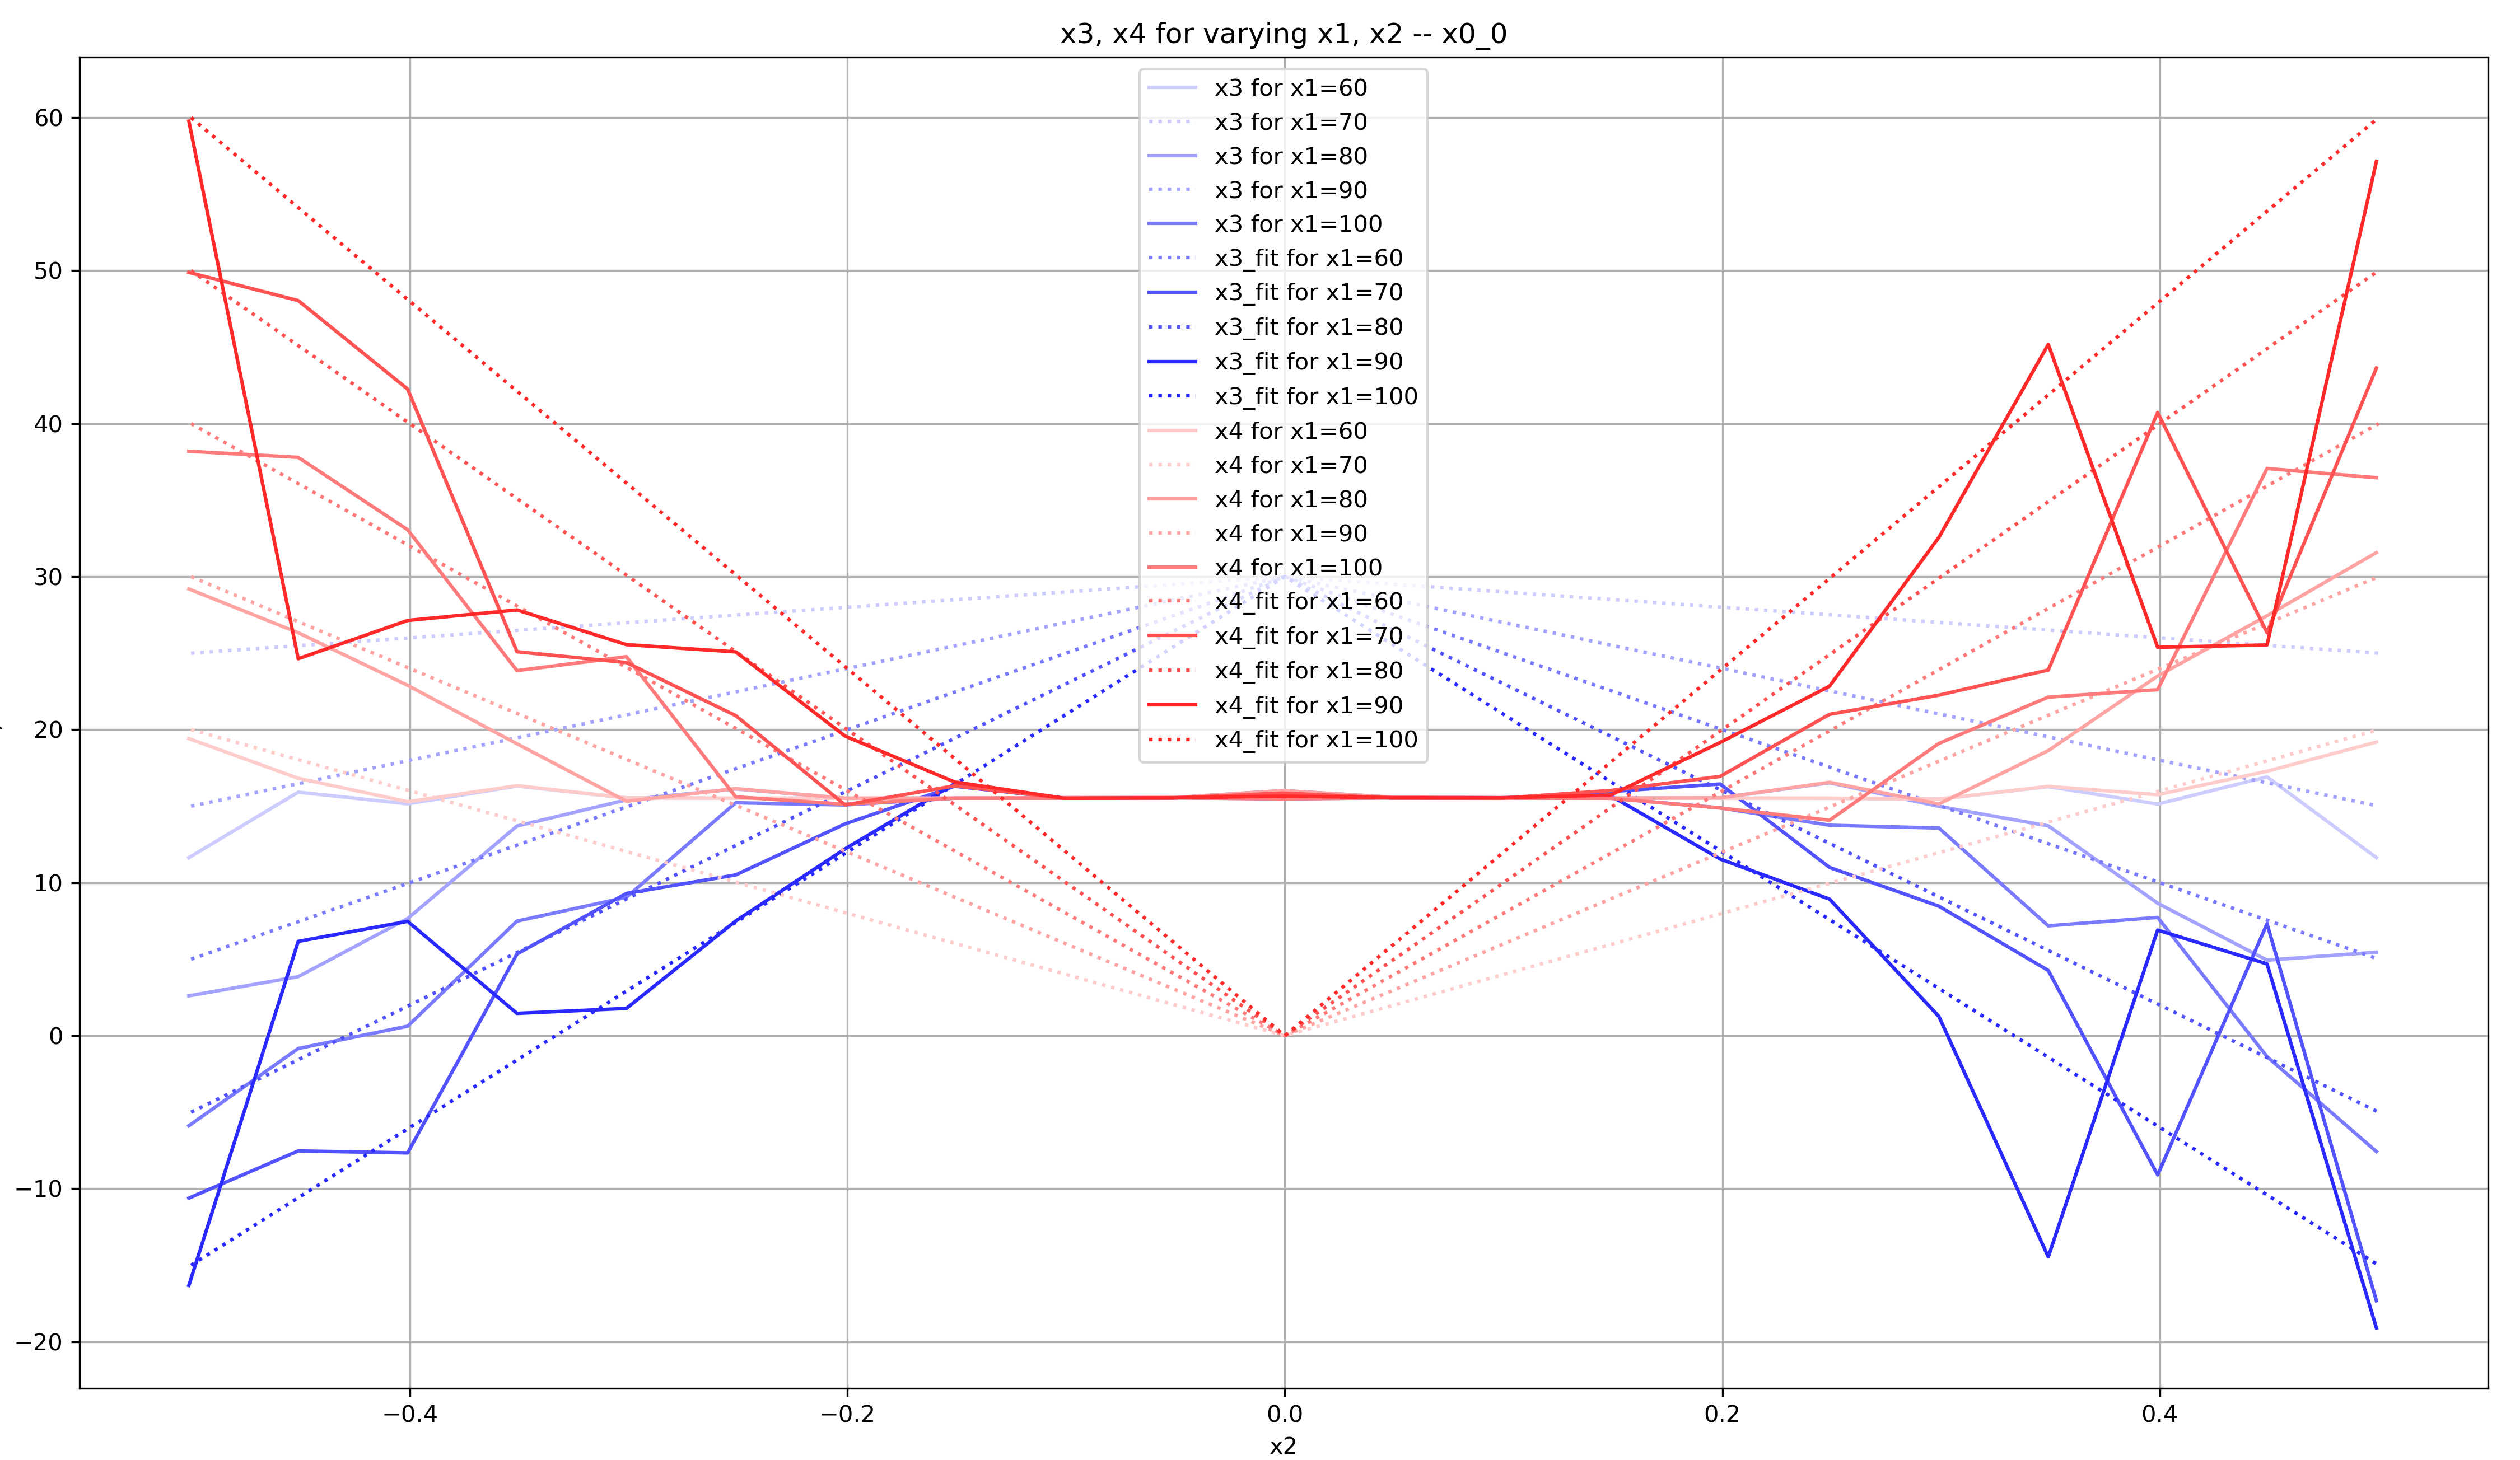
\includegraphics[width=.8\textwidth]{pics/model_3/X3X4.jpg}

		Und somit als Gait Law:
	
		\begin{equation}
		\bm{\alpha} = \begin{bmatrix}
		45 - \frac{x_1}{2} + \bar{f}_0(30 - 2|x_1x_2| + 110|x_2|) + f_0(2|x_1x_2| - 80|x_2|) \\
		45 + \frac{x_1}{2} + \bar{f}_1(30 - 2|x_1x_2| + 110|x_2|) + f_1(2|x_1x_2| - 80|x_2|) \\
		x_1|x_2| \\
		45 - \frac{x_1}{2} + \bar{f}_2(2|x_1x_2| - 80|x_2|) + f_3(30 - 2|x_1x_2| + 110|x_2|) \\
		45 + \frac{x_1}{2} + \bar{f}_3(2|x_1x_2| - 80|x_2|) + f_4(30 - 2|x_1x_2| + 110|x_2|) \\
		\end{bmatrix}
		\end{equation}


\end{itemize}

\subsubsection{Simulation Results}

\begin{itemize}
	\item Gleiche Struktur wie in model 2
	\item Stress ist deutlich kleiner. Drehung allerdings auch. 
\end{itemize}

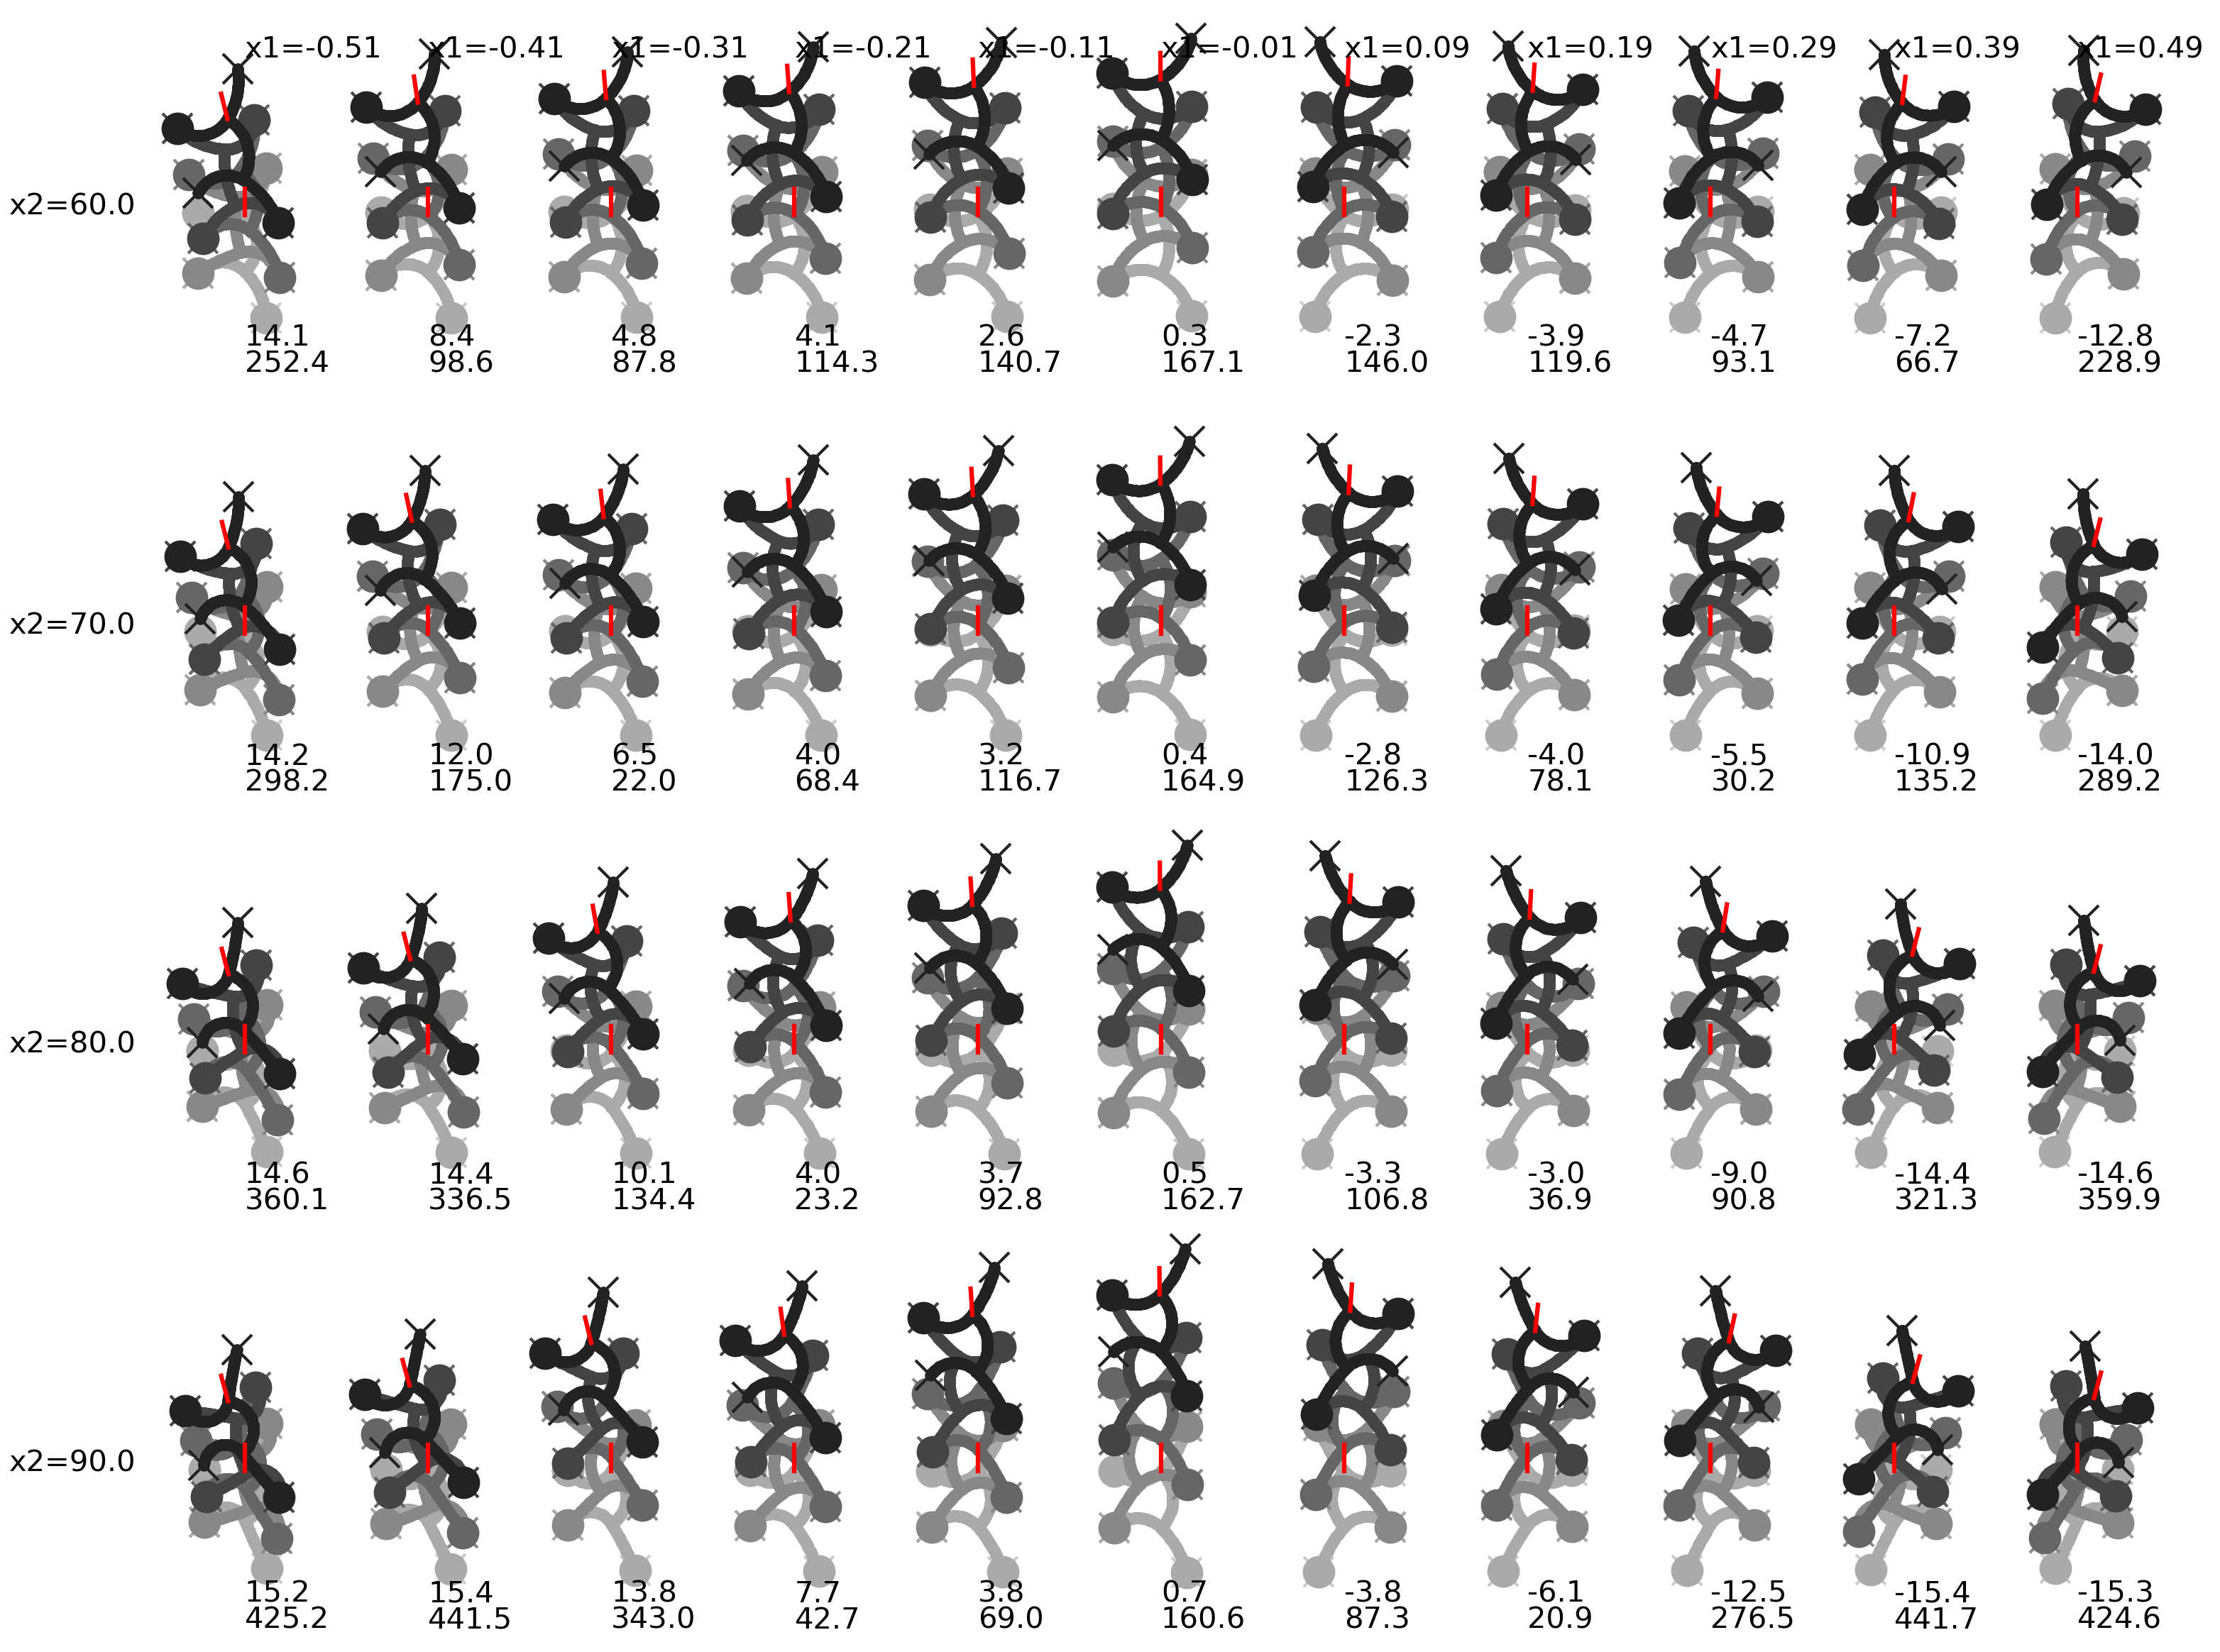
\includegraphics[width=.95\textwidth]{pics/model_3/gait.jpg}

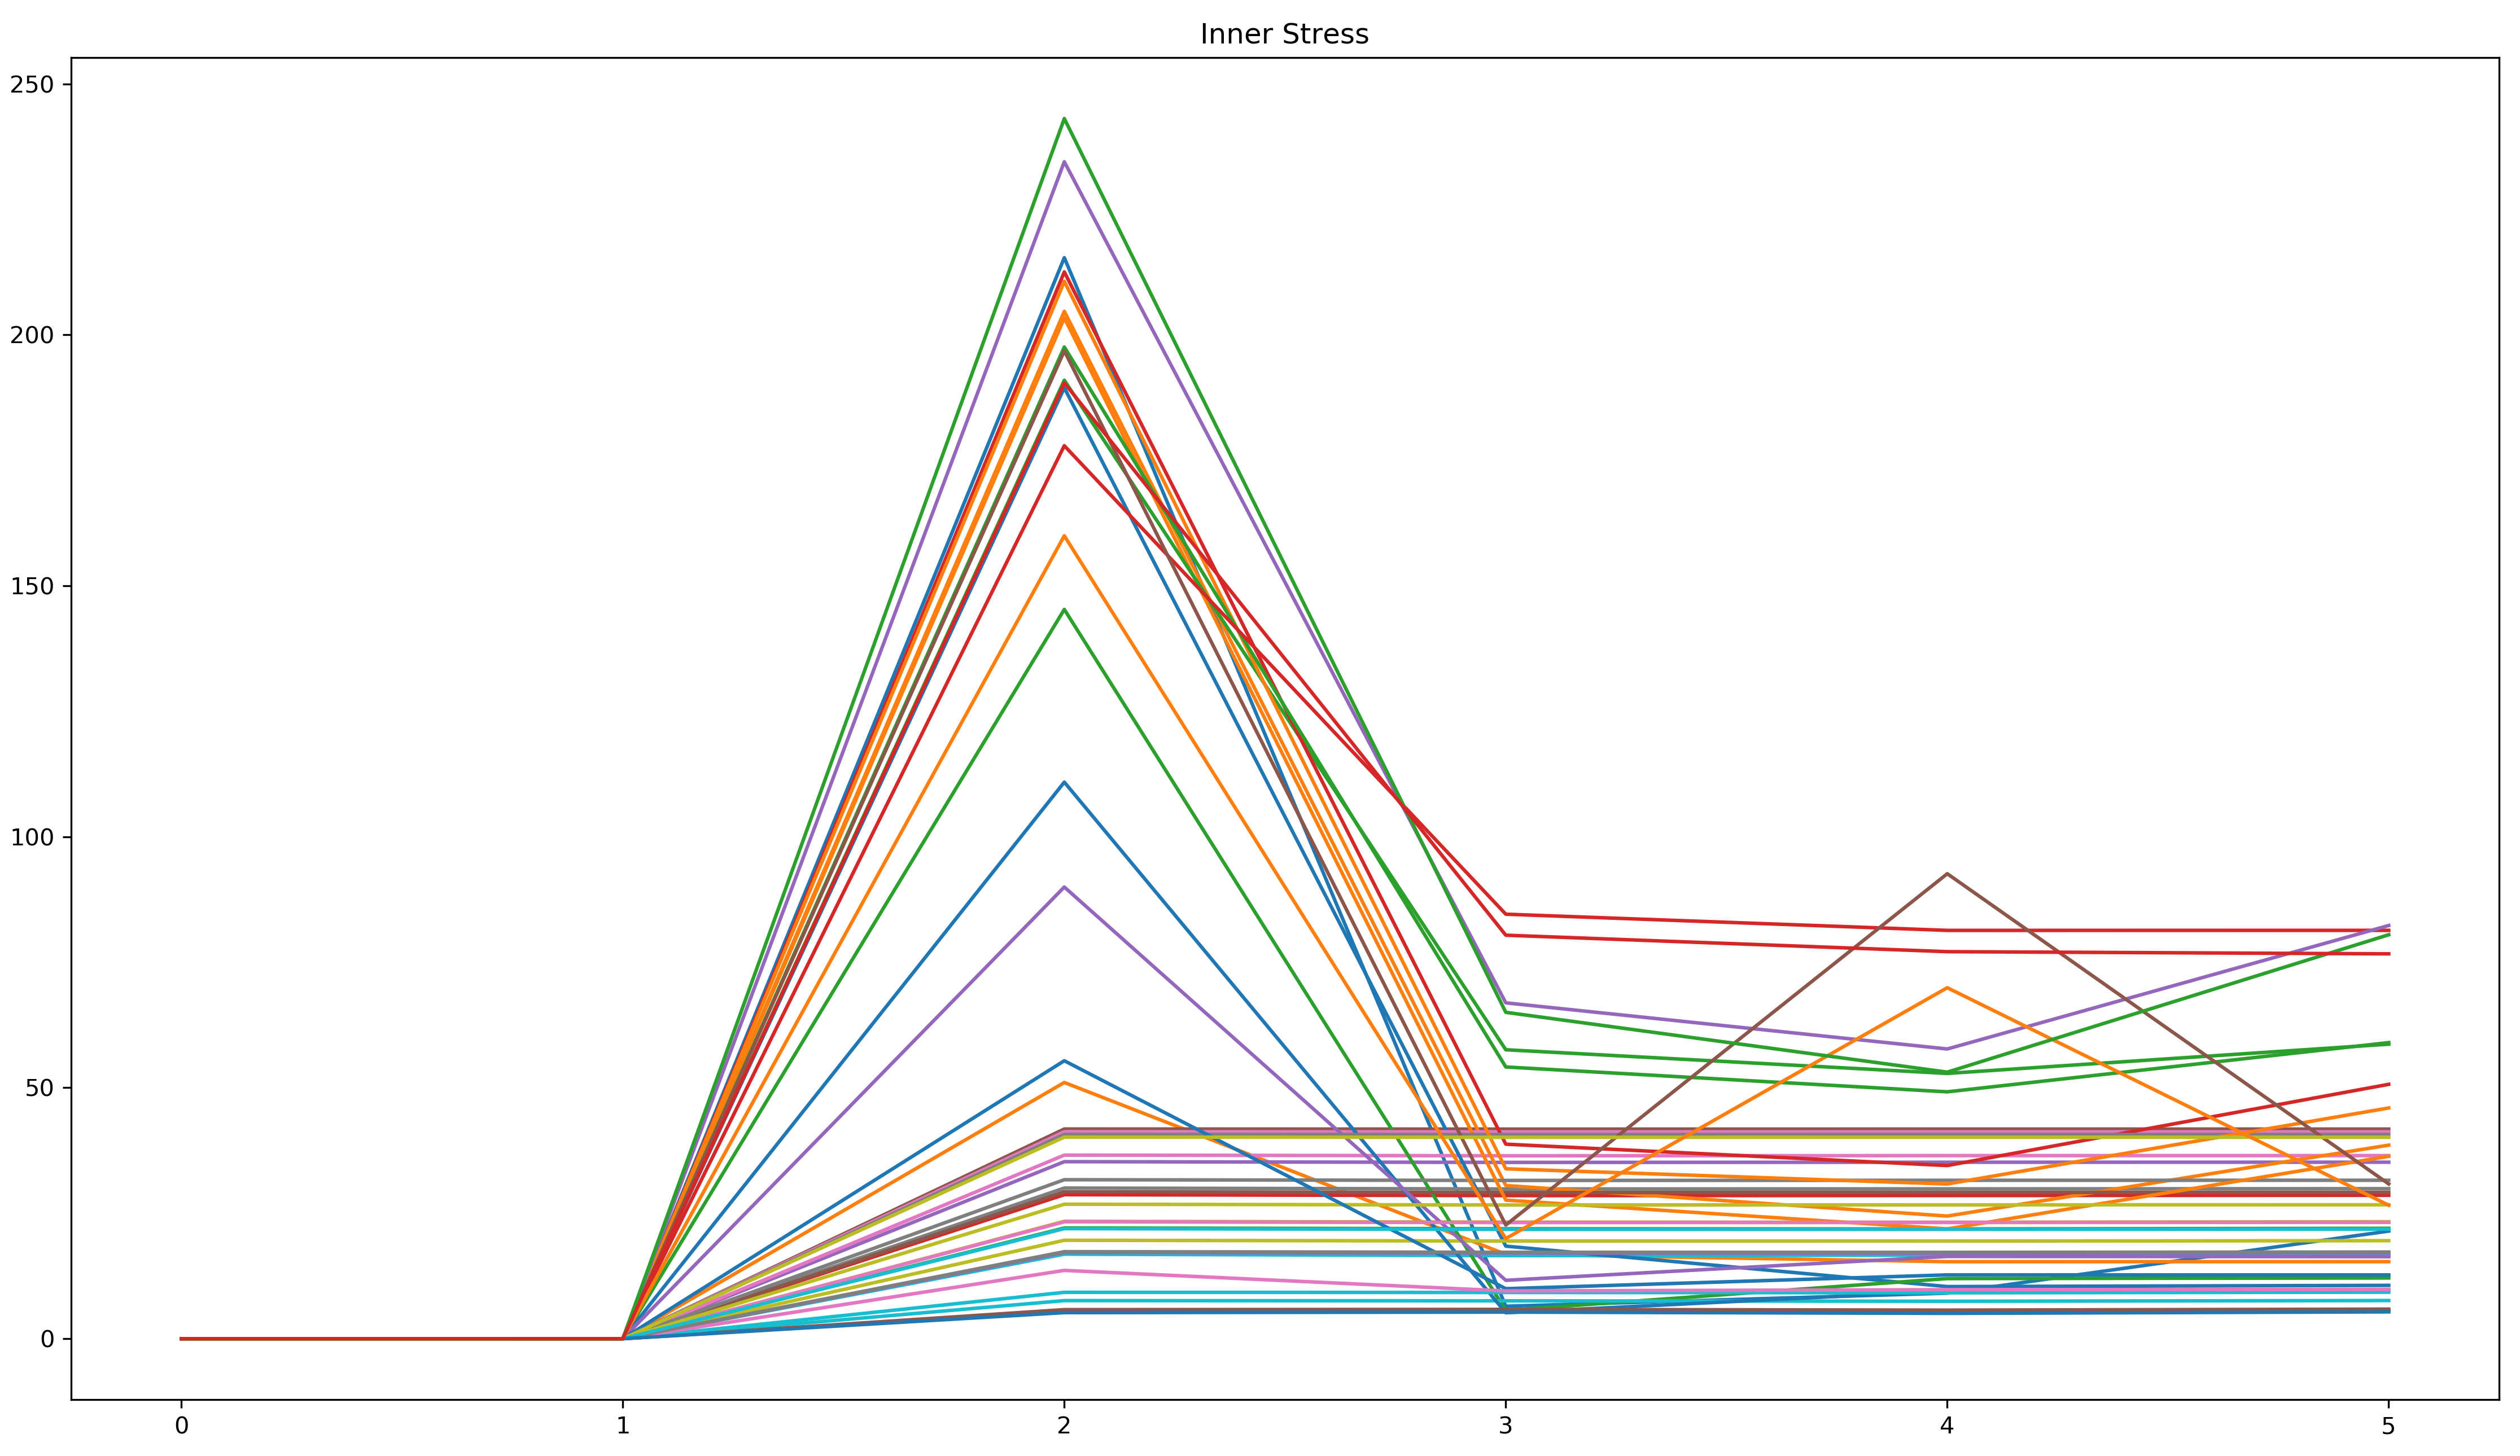
\includegraphics[width=.95\textwidth]{pics/model_3/GeckoBotGaitStress.jpg}





\subsection{Compare model 2 and model 3}

\begin{itemize}
	\item Betrachtet man die beiden unteren Bilder, stellt man fest, dass der dritte Ansatz nicht wirklich erfolgreich war.
	\item Model 2 führt zu besseren Drehungen und kleinerer ineere Spannung. (Zumindest für die betrachtete Zeile ($x_1 = 70$))
\end{itemize}

\begin{tabular}{c}
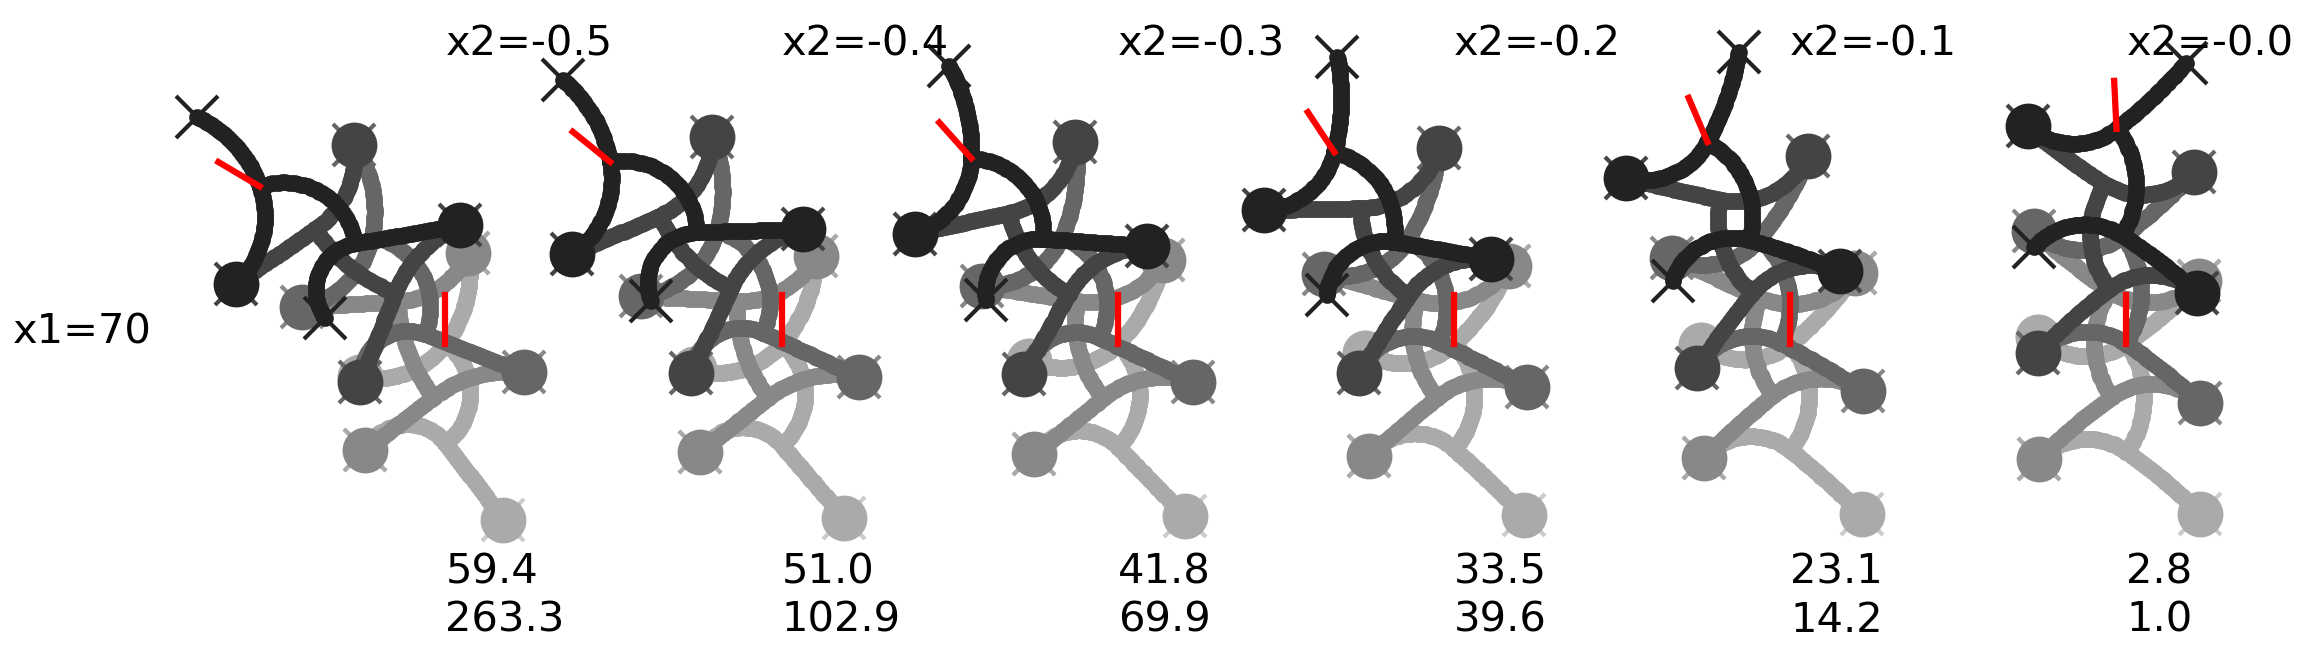
\includegraphics[width=.95\textwidth]{pics/model_2/gait_zoom.jpg} \\
model 2 \\
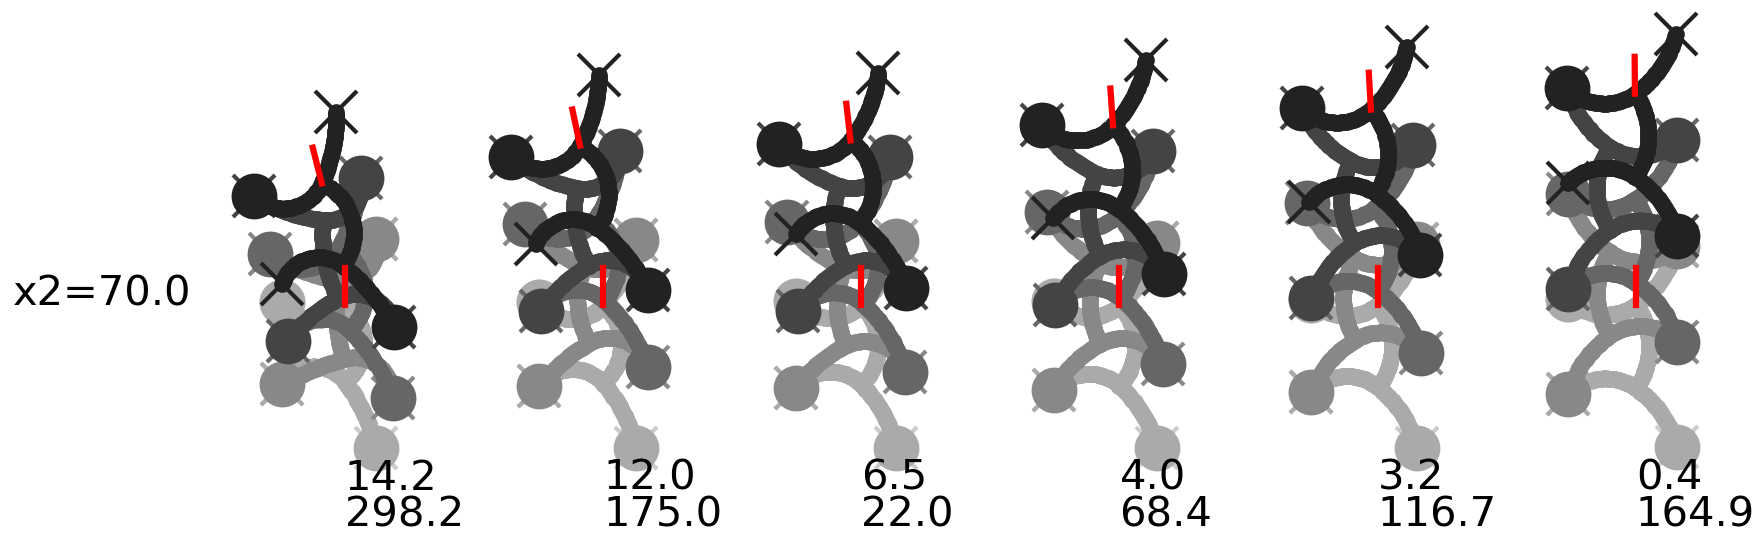
\includegraphics[width=.95\textwidth]{pics/model_3/gait_zoom.jpg} \\
model 3 \\
\end{tabular}

\subsubsection{Conclusion}

\begin{itemize}
	\item Es wird das Gait Law aus Model 2 für den Optimalen Pathplanner gewählt.
\end{itemize}




\section{Optimal PathPlanner based on General Gait Model}

\subsection{Idea}

\begin{itemize}
	\item Wie schon beim SearchTreePathplanner soll die optimale Folgepose berechnet werden.
	\item Optimal in dem Sinne, dass sie den Roboter näher an das Ziel bringt und seine Orientierung so verändert, dass er in die Richtung des Ziels zeigt.
	\item Dieses Mal soll aber nicht aus einer endlichen Anzahl aus vorher definierten möglichen Folgeposen gewählt werden, sondern aus der unendlichen Anzahl aller möglichen Posen.
	\item Das Minimierungsproblem ist ähnlich:
	
	\begin{equation}
	\bm{\rho}_{k+1} = \min_{j} \left( a \frac{d(\bm{\rho_j})}{d_k} + (1-a)\frac{\Delta \varepsilon (\bm{\rho}_j)}{\Delta \varepsilon_k} \right)	
	\end{equation}
	
	\item Mithilfe des analytischen Modells lässt sich die Distanz zum Ziel $d$ und die Orientierungsabweichung $\Delta \varepsilon$ in Abhängigkeit der Schrittweite $x_1$ und des Drehungsmaßes $x_2$ beschreiben.
	
	\item Zur Erinnerung:
	
		\begin{equation}
		\begin{bmatrix}	\delta x \\ \delta y \end{bmatrix} (x_1, x_2) /cycle =\delta \bm{x} (x_1, x_2)= \begin{bmatrix}
		.07x_2 - .29 x_2^2 + .02 x_1x_2 \\
		.02x_1 + .13x_2 - .47x_2^2 \\
		\end{bmatrix}
		\end{equation}
		
%		\begin{equation}
%		\delta \varepsilon (x_1, x_2) / {2~cycle} = -.01x_1 - 21.7 x_2 -.51 x_2^2 - 1.67x_1x_2
%		\end{equation}

		\begin{equation}
		\delta \varepsilon (x_1, x_2) / {cycle} = -.005x_1 - 10.85 x_2 -.255 x_2^2 - .835x_1x_2
		\end{equation}
	
	\item Der Abstand $d$ ergibt sich zu:
	
	\begin{equation}
	d(\bm{\rho}_k, \bar{\bm{x}}, x_1, x_2) = \bigg| \bar{\bm{x}} - \left(\bm{x}_{k} + \bm{R}(\varepsilon_k) \delta \bm{x}(x_1, x_2) \right)\bigg|_2
	\end{equation}	
	
	\item Die Richtungsabweichung $\Delta \varepsilon'$ der Folgepose ergibt sich zu:
	
	\begin{equation}
	\Delta \varepsilon' (\bm{\rho}_k, \bar{\bm{x}}, x_1, x_2) = \measuredangle\left( \bar{\bm{x}} - \left(\bm{x}_{k} + \bm{R}(\varepsilon_k) \delta \bm{x}(x_1,x_2) \right), \bm{R}(\varepsilon_k + \delta \varepsilon (x_1, x_2)) \bm{e}_x \right)
	\end{equation}	
	wobei $\bm{e}_x$ der Einheitsvektor in $x$-Richtung ist.
	
	\item Das Minimierungsproblem lässt sich nun konkretisieren:
	\begin{equation}
	x_{1, \textnormal{opt}}, x_{2, \textnormal{opt}} = \min_{x_1, x_2} \left( a \frac{d(x_1, x_2)}{d_k} + (1-a)\frac{\Delta \varepsilon (x_1, x_2)}{\Delta \varepsilon_k} \right)	
	\end{equation}
	Der nächste Zyklus (i.e. die nächsten zwei Posen) ist damit definiert: 
	\begin{equation}
	\bm{\rho}_{k+1} = [\bm{\alpha}(x_1, x_2),~ \bar{\bm{f}}_k]~,
	\end{equation}
	\begin{equation}
	\bm{\rho}_{k+2} = [\bm{\alpha}(-x_1, x_2),~ {\bm{f}}_k]~,
	\end{equation}
	wobei $\bar{\bm{f}}$ die genau entgegen gesetzte Fixierung von $\bm{f}$ ist.
	
	
\end{itemize}


\subsection{Coordinate Transformation in order to reduce complexity}

\begin{itemize}
	\item Idee: Formulierung des Optimierungsproblems in Koordinaten System des Roboters, Um Komplexität zu verringern.
	\item Messung wird im globalen Kamera system erfolgen, d.h. folgende Größen werden zu verFügung stehen:
	
	\begin{tabular}{ll}
	$^0\bm{x}$ & Position des Roboters im globalen (Kamera-) COS \\
	$^0\bar{\bm{x}}$ & Soll Position im Globalen COS \\
	$^0\varepsilon$ & Orientierung des Roboters im Globalen COS \\
	
	\end{tabular}
	
\end{itemize}

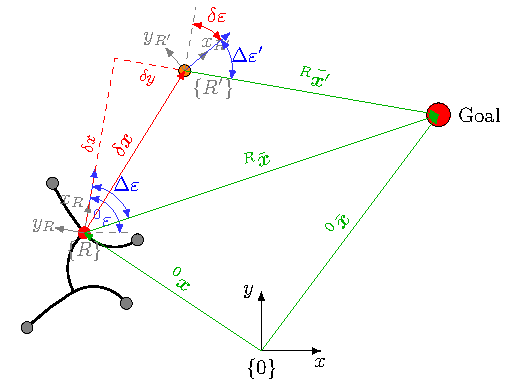
\includegraphics[scale=1]{pics/general_model/model_cost.pdf}

\begin{itemize}
	\item Da das Problem nun im roboterfesten Koordinaten system beschrieben wird, ist der Ortsvektor des Roboters $^R\bm{x} = \bm{0}$.
	\item Den Ortsvector vom Roboter zum Ziel erhält man durch folgende Koordinatentransformation:
	\begin{equation}
	^R\bar{\bm{x}} = \bm{R}(-{^0}\varepsilon)({^0}\bm{\bar{\bm{x}}}-{^0}\bm{x})
	\end{equation}
	\item Die Position der Folgepose $^R\bm{x}'$beschrieben im Roboterfesten COS:
	\begin{equation}
	^R\bm{x}' = \delta \bm{x}(x_1, x_2)
	\end{equation}
	
	\item Der Vektor der von der Folge Pose zum Ziel zeigt, ergibt sich:
	\begin{equation}
		{^R}\bar{\bm{x}}' =  {^R}\bar{\bm{x}} - {^R}\bm{x}'
	\end{equation}	
	
	\item Der Abstand der Folgepose des Roboters beschrieben im Koordinatensystem des Roboters $\{R\}$ zum Ziel $d$ vereinfacht sich nun zu:
	\begin{eqnarray}
		d({^R}\bar{\bm{x}}, x_1, x_2) &=& \big| {^R}\bar{\bm{x}'}\big|_2 \\
		&=& \big| {^R}\bar{\bm{x}} - \delta \bm{x}(x_1, x_2) \big|_2 \\
		&=& \sqrt{ \left({^R}\bar{\bm{x}}_x - \delta \bm{x}_x(x_1, x_2) \right)^2 + \left({^R}\bar{\bm{x}}_y - \delta \bm{x}_y(x_1, x_2) \right)^2 }
	\end{eqnarray}

	\item Und die Richtungsabweichung $\Delta \varepsilon'$ der Folgepose vereinfacht sich nun zu:
	\begin{eqnarray}
	\Delta \varepsilon' ({^R}\bar{\bm{x}}, x_1, x_2) 
	&=& \measuredangle \left( {^R}\bar{\bm{x}} - \delta \bm{x}(x_1,x_2) , {^R}\bm{e}_x \right) - \delta\varepsilon(x_1,x_2) \\
	&=& \atan\left( \frac{{^R}\bar{\bm{x}}_y - \delta\bm{x}_y(x_1,x_2)}{{^R}\bar{\bm{x}}_x - \delta\bm{x}_x(x_1,x_2)}\right) - \delta\varepsilon(x_1,x_2)
	\end{eqnarray}

\end{itemize}


\subsubsection{Explizite Formulierung für mehrer Zyklen}

\includegraphics[scale=1]{pics/general_model/model_cost_2.pdf}

\begin{itemize}
	\item Mit jedem Zyklus dreht sich der Roboter um $\delta \varepsilon$ und verschiebt sich um $\delta \bm{x}$.

	\item Die Position der $(n+1)$-ten Folgepose beschrieben im COS der $(n)$ten Folgepose kann dann rekursiv beschrieben werden:
	\begin{equation}
	{^{R^{(n)}}}\bm{x}^{(n+1)} = \delta \bm{x}(x_1,x_2)
	\end{equation}
	
	\item Den Ortsvector der $(n)$-ten Pose des Roboters zum Ziel (beschrieben im COS der $(n)-$ten Folgepose) erhält man durch folgende Koordinatentransformation der vorhergegangen Pose:
	\begin{equation}
	{^{R^{(n)}}}\bar{\bm{x}}^{(n)} = \bm{R}(-\delta\varepsilon)\left({^{R^{(n-1)}}}\bar{\bm{x}}^{(n-1)}-{^{R^{(n-1)}}}\bm{x}^{(n)}\right)
	\end{equation}
	\item Explizit lässt sich das Formulieren zu:

	\begin{eqnarray}
	{^{R^{(n)}}}\bar{\bm{x}}^{(n)} &=& 
	\bm{R}(-\delta\varepsilon)\left(
	\bm{R}(-\delta\varepsilon) \left( {^{R^{(n-2)}}}\bar{\bm{x}}^{(n-2)} - \delta\bm{x}\right)
	-\delta\bm{x}\right) \\
	&=& 
	\bm{R}^n(-\delta\varepsilon){^R}\bar{\bm{x}}^{(0)} - \sum_{i=0}^n \bm{R}^i(-\delta\varepsilon) \delta \bm{x} \\
	&=& 
	\bm{R}(-n \delta\varepsilon){^R}\bar{\bm{x}}^{(0)} - \sum_{i=0}^n \bm{R}(- i \delta\varepsilon) \delta \bm{x}
	\end{eqnarray}
	
	da mehrfache Rotation um die gleiche Achse und somit $\bm{R}^n(x) = \bm{R}(nx)$

%	\item Der Vektor von der $(n+1)$-ten Pose zum Ziel, beschrieben im COS der $(n)$-ten Pose:
%	\begin{equation}
%	{^{R^{(n)}}}\bar{\bm{x}}^{(n+1)} = {^{R^{(n)}}}\bar{\bm{x}}^{(n)} - {^{R^{(n)}}}\bm{x}^{(n+1)}
%	\end{equation}

	\item Und die Richtungsabweichung $\Delta \varepsilon^{(n)}$ der $(n)$-ten Pose zu:
	\begin{eqnarray}
	\Delta \varepsilon^{(n)} 
	&=& \measuredangle \left( {^{R^{(n)}}}\bar{\bm{x}}^{(n)} , {^{R^{n}}}\bm{e}_x \right) \\
	&=& \atan \left(
	\frac{	{^{R^{(n)}}}\bar{\bm{x}}^{(n)}_y }{
	{^{R^{(n)}}}\bar{\bm{x}}^{(n)}_x}
	\right)
	\end{eqnarray}	
	
	
	\item Nun kann der der Abstand zum Ziel $d_n$ nach $n$ Zyklen mit dem zu $\delta\bm{x} = [\delta x, \delta y, \delta \varepsilon]^\top$ korrespondierenden Laufmuster formuliert werden:
	\begin{equation}
	d_n({^R}\bar{\bm{x}}, \delta\bm{x}) = \bigg| \bm{R}(-n \delta\varepsilon){^R}\bar{\bm{x}} - \sum_{i=0}^n \bm{R}(- i \delta\varepsilon) \delta \bm{x} \bigg|_2
	\end{equation}
	
\end{itemize}

\subsection{Simplified Optimization Problem}

\begin{itemize}

	\item Da die Richtungsabweichung $\Delta \varepsilon$ im der Abstandsformel für mehrere Zyklen schon implizit enthalten ist, kann das Minimierungsproblem nun drastisch vereinfacht werden (die Funktion wird quadriert, um die Wurzel zu beseitigen und die Ableitung zu vereinfachen):
	
	\begin{equation}
	x_{1, \textnormal{opt}}, x_{2, \textnormal{opt}} = \min_{x_1, x_2} d^2_n({^R}\bar{\bm{x}}, \delta\bm{x})
	\end{equation}
	
	\item Zur Lösung des Optimierungsproblems ist die Jacobi-Matrix sehr hilfreich:
	\begin{equation}
	\bm{{J}} = \begin{bmatrix}
		\frac{\delta f}{\delta x_1} &
		\frac{\delta f}{\delta x_2}
	\end{bmatrix}
	\end{equation}

	\item Möge die Suche nach der Jacobi Matrix beginnen
\end{itemize}

\subsubsection{Calculation of Jacobian}



\paragraph{Ableitung der Trigonometrischen Summe in einer Dimension}

Als Euler'sche Formulierung

\begin{equation}
\sum_{k=0}^n \sin(k\delta_{\varepsilon}) = 
\frac{i \left(- e^{i \delta_{\varepsilon} n} + 1\right) \left(- e^{i \delta_{\varepsilon} \left(n + 1\right)} + 1\right) e^{- i \delta_{\varepsilon} n}}{2 \left(- e^{i \delta_{\varepsilon}} + 1\right)}
\end{equation}

Ableitung:

\begin{equation}
\frac{\left(- n e^{i \delta_{\varepsilon}} + n e^{2 i \delta_{\varepsilon} \left(n + 1\right)} - n e^{i \delta_{\varepsilon} \left(2 n + 1\right)} + n - e^{i \delta_{\varepsilon}} + 2 e^{i \delta_{\varepsilon} \left(n + 1\right)} - e^{i \delta_{\varepsilon} \left(2 n + 1\right)}\right) e^{- i \delta_{\varepsilon} n}}{2 \left(e^{2 i \delta_{\varepsilon}} - 2 e^{i \delta_{\varepsilon}} + 1\right)}
\end{equation}

Laut Formelsammlung (BFS39):

\begin{equation}
\sum_{k=0}^n \sin(k\delta_{\varepsilon}) = 
\frac{\sin{\left (\frac{\delta_{\varepsilon} n}{2} \right )} \sin{\left (\frac{\delta_{\varepsilon} \left(n + 1\right)}{2} \right )}}{\sin{\left (\frac{\delta_{\varepsilon}}{2} \right )}}
\end{equation}

Ableitung

\begin{equation}
\frac{n \cos{\left (\delta_{\varepsilon} n \right )} - n \cos{\left (\delta_{\varepsilon} \left(n + 1\right) \right )} + \cos{\left (\delta_{\varepsilon} n \right )} - 1}{2 \left(- \cos{\left (\delta_{\varepsilon} \right )} + 1\right)}
\end{equation}


\paragraph{Partielle Ableitung der Trigonometrischen Summe}

Euler:
\begin{equation}
\frac{i \left(- e^{i n \left(c_{0} x_{1} + c_{1} x_{2} + c_{2} x_{2}^{2} + c_{3} x_{1} x_{2}\right)} + 1\right) \left(- e^{i \left(n + 1\right) \left(c_{0} x_{1} + c_{1} x_{2} + c_{2} x_{2}^{2} + c_{3} x_{1} x_{2}\right)} + 1\right) e^{- i n \left(c_{0} x_{1} + c_{1} x_{2} + c_{2} x_{2}^{2} + c_{3} x_{1} x_{2}\right)}}{2 \left(- e^{i \left(c_{0} x_{1} + c_{1} x_{2} + c_{2} x_{2}^{2} + c_{3} x_{1} x_{2}\right)} + 1\right)}
\end{equation}
Ableitung:
\begin{equation}
\frac{\delta}{\delta x_1} =
- \frac{\left(c_{0} + c_{3} x_{2}\right) \left(\left(n \left(e^{i n \left(c_{0} x_{1} + c_{1} x_{2} + c_{2} x_{2}^{2} + c_{3} x_{1} x_{2}\right)} + 1\right) \left(- e^{i \left(n + 1\right) \left(c_{0} x_{1} + c_{1} x_{2} + c_{2} x_{2}^{2} + c_{3} x_{1} x_{2}\right)} + 1\right) + \left(n + 1\right) \left(- e^{i n \left(c_{0} x_{1} + c_{1} x_{2} + c_{2} x_{2}^{2} + c_{3} x_{1} x_{2}\right)} + 1\right) \left(e^{i \left(n + 1\right) \left(c_{0} x_{1} + c_{1} x_{2} + c_{2} x_{2}^{2} + c_{3} x_{1} x_{2}\right)} + 1\right)\right) \left(e^{i \left(c_{0} x_{1} + c_{1} x_{2} + c_{2} x_{2}^{2} + c_{3} x_{1} x_{2}\right)} - 1\right) e^{\frac{i \left(2 n + 2\right) \left(c_{0} x_{1} + c_{1} x_{2} + c_{2} x_{2}^{2} + c_{3} x_{1} x_{2}\right)}{2}} + \left(e^{i \left(c_{0} x_{1} + c_{1} x_{2} + c_{2} x_{2}^{2} + c_{3} x_{1} x_{2}\right)} + 1\right) \left(e^{i n \left(c_{0} x_{1} + c_{1} x_{2} + c_{2} x_{2}^{2} + c_{3} x_{1} x_{2}\right)} - 1\right) \left(e^{i \left(n + 1\right) \left(c_{0} x_{1} + c_{1} x_{2} + c_{2} x_{2}^{2} + c_{3} x_{1} x_{2}\right)} - 1\right) e^{i \left(n + 1\right) \left(c_{0} x_{1} + c_{1} x_{2} + c_{2} x_{2}^{2} + c_{3} x_{1} x_{2}\right)}\right) e^{- i \left(2 n + 1\right) \left(c_{0} x_{1} + c_{1} x_{2} + c_{2} x_{2}^{2} + c_{3} x_{1} x_{2}\right)}}{4 \left(e^{i \left(c_{0} x_{1} + c_{1} x_{2} + c_{2} x_{2}^{2} + c_{3} x_{1} x_{2}\right)} - 1\right)^{2}}
\end{equation}

\begin{equation}
\frac{\delta}{\delta x_2} =
- \frac{\left(\left(n \left(e^{i n \left(c_{0} x_{1} + c_{1} x_{2} + c_{2} x_{2}^{2} + c_{3} x_{1} x_{2}\right)} + 1\right) \left(- e^{i \left(n + 1\right) \left(c_{0} x_{1} + c_{1} x_{2} + c_{2} x_{2}^{2} + c_{3} x_{1} x_{2}\right)} + 1\right) + \left(n + 1\right) \left(- e^{i n \left(c_{0} x_{1} + c_{1} x_{2} + c_{2} x_{2}^{2} + c_{3} x_{1} x_{2}\right)} + 1\right) \left(e^{i \left(n + 1\right) \left(c_{0} x_{1} + c_{1} x_{2} + c_{2} x_{2}^{2} + c_{3} x_{1} x_{2}\right)} + 1\right)\right) \left(e^{i \left(c_{0} x_{1} + c_{1} x_{2} + c_{2} x_{2}^{2} + c_{3} x_{1} x_{2}\right)} - 1\right) e^{\frac{i \left(2 n + 2\right) \left(c_{0} x_{1} + c_{1} x_{2} + c_{2} x_{2}^{2} + c_{3} x_{1} x_{2}\right)}{2}} + \left(e^{i \left(c_{0} x_{1} + c_{1} x_{2} + c_{2} x_{2}^{2} + c_{3} x_{1} x_{2}\right)} + 1\right) \left(e^{i n \left(c_{0} x_{1} + c_{1} x_{2} + c_{2} x_{2}^{2} + c_{3} x_{1} x_{2}\right)} - 1\right) \left(e^{i \left(n + 1\right) \left(c_{0} x_{1} + c_{1} x_{2} + c_{2} x_{2}^{2} + c_{3} x_{1} x_{2}\right)} - 1\right) e^{i \left(n + 1\right) \left(c_{0} x_{1} + c_{1} x_{2} + c_{2} x_{2}^{2} + c_{3} x_{1} x_{2}\right)}\right) \left(c_{1} + 2 c_{2} x_{2} + c_{3} x_{1}\right) e^{- i \left(2 n + 1\right) \left(c_{0} x_{1} + c_{1} x_{2} + c_{2} x_{2}^{2} + c_{3} x_{1} x_{2}\right)}}{4 \left(e^{i \left(c_{0} x_{1} + c_{1} x_{2} + c_{2} x_{2}^{2} + c_{3} x_{1} x_{2}\right)} - 1\right)^{2}}
\end{equation}

Normal:
\begin{equation}
\frac{\sin{\left (\frac{n \left(c_{0} x_{1} + c_{1} x_{2} + c_{2} x_{2}^{2} + c_{3} x_{1} x_{2}\right)}{2} \right )} \sin{\left (\frac{\left(n + 1\right) \left(c_{0} x_{1} + c_{1} x_{2} + c_{2} x_{2}^{2} + c_{3} x_{1} x_{2}\right)}{2} \right )}}{\sin{\left (\frac{c_{0} x_{1}}{2} + \frac{c_{1} x_{2}}{2} + \frac{c_{2} x_{2}^{2}}{2} + \frac{c_{3} x_{1} x_{2}}{2} \right )}}
\end{equation}


\end{document}